% ch15a Quantum Hall and other topological states, part a (书页 317-342 / 分册p001-026)
% 第15章 Quantum Hall and other topological states
\chapter{量子霍尔与其他拓扑态}

当电子气体被限制在两种半导体的界面上运动、且沿垂直于该平面的方向施加磁场时，在足够低的温度下会出现一种新的物质态（TSG1982）。这种物质态在凝聚态物理学中是独一无二的：它对所有激发都具有能隙，并表现出分数统计（fractional statistics）。它通常被称为不可压缩量子液体（incompressible quantum liquid），或劳夫林液体（L1983），以这一态的构建者命名。虽然劳夫林态是由电子间的相互排斥所中介的，但正是大的垂直磁场的存在导致了这一新多体态的不可压缩性。它的前身是整数量子霍尔态。在这一态中，无序与磁场协同作用，把相关的电荷输运限制在样品边缘附近的窄带内。这种边缘电流的新颖之处在于它以 $e^{2}/h$ 的整数倍量子化（KDP1980）。劳夫林态中相应的电流仍是量子化的，但以 $e^{2}/h$ 的分数倍量子化。本章将给出理解这两种效应的基本物理所需的现象学描述与数学描述。

正如我们将看到的，拓扑是量子霍尔效应不可分割的一部分。无论几何形状如何，也无论哈密顿量如何平滑变化，电导的量子化只取决于具有确定手性（chirality）的边缘态的存在。虽然在磁场存在下边缘态很容易得到理解，但这种破坏时间反演的场并非必需。正是认识到边缘态可以在时间反演对称性存在时出现，才催生了拓扑绝缘体（topological insulator）这一新领域（KM2005a; KM2005b; TFK2008; HK2010; BHZ2006; R2009; MB2007; X2009; Z2009; QHZ2008; QZ2010; K2007; BZ2006）。与量子霍尔系统的关键差别在于：这里的边缘态必然双重简并，每个自旋各对应一个，而量子霍尔效应中只有单一的载流态。本章将给出一个简单模型，用以捕捉在一原本绝缘的样品中这类拓扑保护态的本质。

\section{什么是量子霍尔效应？}

要理解霍尔效应的“量子”究竟为何意，我们必须先定义霍尔电压的概念（H1879）。为此，考虑一块导电金属板，其中电流 $I$ 沿 $x$ 方向流动。如图 15.1(a) 所示，电流沿 $x$ 轴产生电压降、电场 $E_{x}$ 和电流密度 $j_{x}$。我们假设电流密度与电场之间呈线性关系（欧姆定律）
\begin{equation*}
j_{x}=\sigma_{0}E_{x},
\end{equation*}
比例常数由第 10 章导出的德鲁德（Drude）电导给出。在沿 $z$ 轴向上取向的磁场存在时，电子将在洛伦兹力的作用下向负 $y$ 方向偏折（图 15.1(b)）。若样品在 $y$ 方向无限延伸，电流将不再单纯沿 $x$ 轴方向；电子将以相对 $x$ 轴成某一角度的方式运动，该角度定义了霍尔角（Hall angle）。然而，若样品在 $y$ 方向受限，被磁场偏折的电子最终会撞到样品的边缘。当电子在边缘积累时，会产生一个指向正 $y$ 方向的电场 $E_{y}$。当电场 $E_{y}$ 大到足以抵消洛伦兹力时，电子在样品边缘的进一步积累便告停止。平衡时洛伦兹力被抵消（图 15.1(c)）意味着电子将纯粹沿 $x$ 轴输运。促成这种抵消的附加电场 $E_{y}$ 可以简单地看作一种感应场，它由边界处电荷的磁通所产生。正是这个 $E_{y}$ 场被称为霍尔场。在均匀系统的平衡态中，霍尔场垂直于电流。对于宽度为 $W$ 的严格二维样品，霍尔电压 $V_{\mathrm{H}}$ 通过 $E_{y}=V_{\mathrm{H}}/W$ 与霍尔场相联系。总电流为 $I=Wj_{x}$。

\begin{figure}[H]\centering
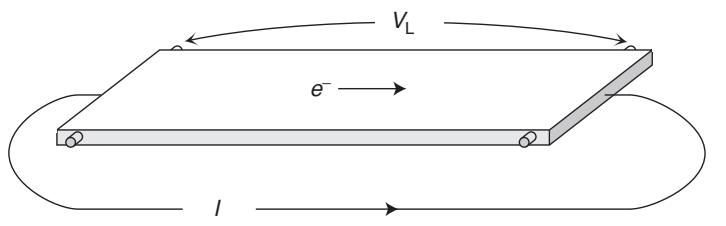
\includegraphics[width=0.60\textwidth]{figs/ch15/fig_15.1_a.jpg}\\[4pt]
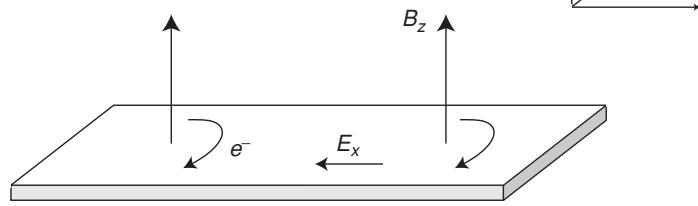
\includegraphics[width=0.60\textwidth]{figs/ch15/fig_15.1_b.jpg}\\[4pt]
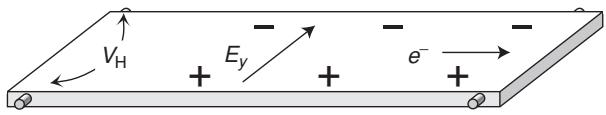
\includegraphics[width=0.60\textwidth]{figs/ch15/fig_15.1_c.jpg}
\caption*{图 15.1\quad (a) 霍尔效应的标准几何安排。电流 $I$ 沿 $x$ 方向流过薄样品，沿 $x$ 轴产生电压降和电场 $E_{x}$。样品被沿正 $z$ 方向的均匀磁场 $B_{z}$ 穿过。(b) 电子为响应磁场而在 $y$ 方向上发生的侧向运动。电子在材料的一个面上积累，产生横向电场 $E_{y}$。(c) 正离子过剩不断建立，直到霍尔场 $E_{y}$ 抵消洛伦兹力。}\label{fig:auto:15.1}
\end{figure}

为理解 $E_{y}$ 作为磁场的函数如何变化，我们发展一个半经典或高温理论。在这一区间，我们可以通过应用牛顿第二定律
\begin{equation*}
F=-e\left(\mathbf{E}+\frac{1}{c}\mathbf{v}\times\mathbf{B}\right)\tag{15.1}
\end{equation*}
到受限的金属板上来确定霍尔场的量级，其中 $\mathbf{v}$ 与 $\mathbf{B}$ 分别是电子速度和磁场。$y$ 方向上力的抵消要求
\begin{equation*}
E_{y}=\frac{v_{x}B_{z}}{c}.\tag{15.2}
\end{equation*}
如同在第 10 章中那样，我们对电子速度采用弛豫时间近似，$v_{x}=-eE_{x}\tau/m$，其中 $\tau$ 为碰撞时间。本问题中另一个基本时间尺度由回旋频率（cyclotron frequency）确定，
\begin{equation*}
\omega_{\mathrm{c}}\equiv\frac{eB_{z}}{mc}.\tag{15.3}
\end{equation*}
借助弛豫时间近似，我们可以用回旋频率把霍尔场
\begin{equation*}
E_{y}=-\omega_{\mathrm{c}}\tau E_{x}\tag{15.4}
\end{equation*}
改写出来。由于电流密度
\begin{equation*}
j_{x}=\frac{e^{2}\tau\rho E_{x}}{m},\tag{15.5}
\end{equation*}
正比于 $\tau E_{x}$，故由
\begin{equation*}
\rho_{\mathrm{H}}=\frac{E_{y}}{I}=\frac{E_{y}}{Wj_{x}}\tag{15.6}
\end{equation*}
定义的横向电阻率与弛豫时间无关。然而在霍尔实验中，直接测量的量是横向电压 $V_{\mathrm{H}}$ 和纵向电压 $V_{\mathrm{L}}=E_{x}L$，其中 $L$ 是电压变化 $V_{\mathrm{L}}$ 所跨越的纵向距离。因此，在霍尔效应中，考虑电阻而非电阻率更为方便。霍尔电阻
\begin{equation*}
R_{\mathrm{H}}=\frac{V_{\mathrm{H}}}{I}=\frac{WE_{y}}{Wj_{x}}=-\frac{B_{z}}{ec\rho},\tag{15.7}
\end{equation*}
与所加磁场呈线性关系，而纵向电阻
\begin{equation*}
R_{\mathrm{L}}=\frac{V_{\mathrm{L}}}{I}=\frac{LE_{x}}{Wj_{x}}=\frac{L}{W}\frac{1}{\sigma_{0}},\tag{15.8}
\end{equation*}
则与磁场无关。实验上，这些关系与霍尔（Hall）1879 年的测量符合得很好（H1879）。注意，我们这里算出的 $R_{\mathrm{H}}$ 与电子散射过程的细节无关。一般而言，对这类过程存在弱的依赖。

1980 年，冯·克利青（von Klitzing）及其合作者（KDP1980）注意到，在足够高的磁场和超低温度下，电阻明显偏离式 (15.7) 与式 (15.8) 所给的数值。他们在硅 MOSFET 中限制于 $\mathrm{SiO}_{2}$ 与 Si 界面处的二维电子气上完成了这些非凡的实验。他们发现，随磁场增大，霍尔电压呈现出明显的平坦区域即平台（plateau），且平台在不同样品之间高度可重复，如图 15.2 所示。由平台区处霍尔电压的数值，他们推断霍尔电导（电阻的倒数）必定以 $e^{2}/h$ 为单位量子化。电导按
\begin{equation*}
\sigma_{\mathrm{H}}=-\frac{ne^{2}}{h},\tag{15.9}
\end{equation*}
（$n$ 为整数）的形式量子化，其精度达 $10^{7}$ 分之一。同样令人惊讶的是纵向电阻的行为。他们发现纵向电阻恰在霍尔平台处消失，表明无耗散输运的开始。量子化与完美导电同时出现，表明这些实验的核心有着十分根本的东西。在更高的磁场和更低的温度下，崔琦（Tsui）、斯托默（Störmer）和戈萨德（Gossard）（TSG1982）发现霍尔电压的平台区远比原先认为的丰富。他们发现，当电导是 $e^{2}/h$ 的分数倍时也会出现平台区，这表明存在分数电荷的激发。我们将证明，整数霍尔效应可以简单地理解为边缘电流的量子化，而分数效应则源自一种根本上全新的关联多体态——劳夫林态（L1983）。

\begin{figure}[H]\centering
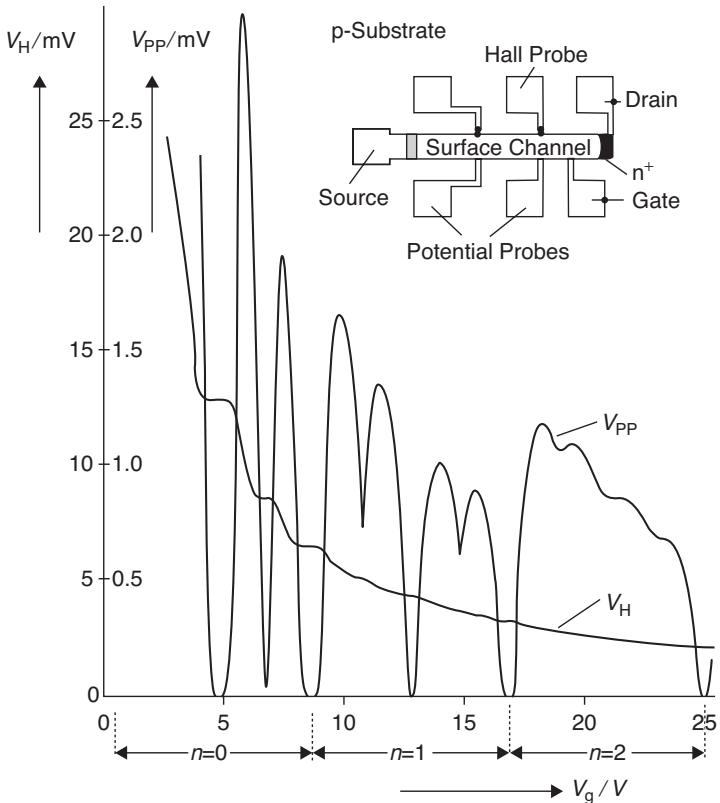
\includegraphics[width=0.52\textwidth]{figs/ch15/fig_15.2.jpg}
\caption*{图 15.2\quad 在 $T=1.5\,$K 下，霍尔电压 $V_{\mathrm{H}}$ 与电势探针之间的电势降 $V_{\mathrm{pp}}$ 随栅压 $V_{\mathrm{g}}$ 的变化。磁场固定在 18 T，源漏电流为 $1\,\mu\mathrm{A}$。插图为器件的俯视图，其长度 $L=400\,\mu\mathrm{m}$，宽度 $W=50\,\mu\mathrm{m}$，电势探针间距 $L_{\mathrm{pp}}=130\,\mu\mathrm{m}$。霍尔平台出现在每个朗道能级填充的整数取值处，以指标 $n$ 标示。在霍尔电压的平台处，纵向电压趋于零，表明存在无耗散输运。}\label{fig:auto:15.2}
\end{figure}

\section{朗道能级}

作为开始，我们求解描述电子在被垂直磁场穿过的平面内运动的波函数。遵循朗道的原始处理，我们取向矢势
\begin{equation*}
A_{y}=Bx,\quad A_{x}=0,\tag{15.10}
\end{equation*}
沿 $y$ 方向，单粒子薛定谔方程取如下形式
\begin{equation*}
-\frac{\hbar^{2}}{2m}\left(\partial_{x}^{2}+\left(\partial_{y}-\mathrm{i}eBx/\hbar c\right)^{2}\right)\psi(x,y)=E\psi(x,y).\tag{15.11}
\end{equation*}
这一规范选择最便于描述整数量子霍尔效应中的输运。然而，在分数量子霍尔效应的语境下，我们会发现采用对称规范更为便利，在该规范中
\begin{equation*}
\mathbf{A}=\frac{B}{2}\left(y\widehat{x}-x\widehat{y}\right).\tag{15.12}
\end{equation*}
在对称规范中，沿 $z$ 方向施加磁场导致沿 $x$、$y$ 两轴均为谐振子问题。因此，一旦求得由式 (15.10) 描述的较简单问题的解，此问题便易于解决。

$y$ 方向的平移不变性提示我们把波函数写成
\begin{equation*}
\psi_{n,k}(x,y)=\mathrm{e}^{\mathrm{i}ky}f_{n}(x).\tag{15.13}
\end{equation*}
把 $\psi_{n,k}(x,y)$ 代入式 (15.11) 可知，$f_{n}(x)$ 是谐振子方程
\begin{equation*}
\frac{\hbar\omega_{\mathrm{c}}}{2}\left(-\ell^{2}\partial_{x}^{2}+\left(x/\ell-\ell k\right)^{2}\right)f_{n}(x)=\epsilon_{n}f_{n}(x)\tag{15.14}
\end{equation*}
的解。其中，与回旋频率不同，长度尺度
\begin{equation*}
\ell\equiv\sqrt{\frac{\hbar c}{eB}}=\frac{250\,\text{\AA}}{\sqrt{B}}\tag{15.15}
\end{equation*}
不依赖于有效质量，且完全通过改变磁场来改变。这个量被称为磁性长度（magnetic length），在 $B=1\,$T 的场中 $\ell$ 约为 250\,\AA。由谐振子基态出发，我们生成一族高斯型波函数
\begin{equation*}
\psi_{n,k}(x,y)=\mathrm{e}^{\mathrm{i}ky}H_{n}(x/\ell-\ell k)\,\mathrm{e}^{-\frac{(x-x_{k})^{2}}{2\ell^{2}}}\tag{15.16}
\end{equation*}
它们沿 $y$ 方向延展，但在 $x$ 方向局域，并中心位于 $x_{k}=\ell^{2}k$。在式 (15.16) 中，$H_{n}$ 是厄米多项式。每个以 $n$ 标记的态称为一个朗道能级。每个朗道能级的能量为
\begin{equation*}
\epsilon_{n}=\hbar\omega_{\mathrm{c}}\left(n+\frac{1}{2}\right)\tag{15.17}
\end{equation*}
因而与 $k$ 无关。结果，每个朗道能级由若干等能态组成。对于 $B=1\,$T 的场，零点能为 $10^{-4}\,\mathrm{eV}$ 的量级，即 1.34 K。如果温度低于由零点能确定的温度，我们就会看到分立朗道能级中量子化的效应。我们对 1.34 K 的估计略有不准，因为我们没有使用半导体的有效质量。对于 GaAs，$m^{*}=0.06m$；因此零点能增大 16 倍，朗道能级量子化效应在实验上可观察的温度也同样提高 16 倍。

由于这种简并，每个朗道能级可以容纳许多电子。简并度由能在同一朗道能级内生成一个态的彼此不同的 $k$ 值的数目决定。我们注意到，组成每个朗道能级的态中心位于 $x_{k}=\ell^{2}k$，其中 $k$ 可取与系统在 $y$ 方向受限相一致的一系列数值。设 $L$ 与 $W$ 分别是样品在 $x$ 与 $y$ 方向的空间尺度。若把波矢 $k$ 写成
\begin{equation*}
k_{m}=\frac{2\pi m}{W},\tag{15.18}
\end{equation*}
其中 $m$ 为整数，则每个朗道能级容许的最大态数可由求解条件 $L=\ell^{2}k_{N_{\mathrm{max}}}$ 得到，或等价地
\begin{equation*}
N_{\mathrm{max}}=\frac{LW}{2\pi\ell^{2}}=\frac{eBLW}{hc}.\tag{15.19}
\end{equation*}
这个表达式的右端有一个简单的物理解释。每个朗道能级内的总磁通是磁场与样品面积的乘积 $BLW$。这个量必等于每个能级中的电子数乘以磁通量子 $hc/e$。于是我们看到，$N_{\mathrm{max}}$ 也就是每个朗道能级中的电子数。因此，我们对每个朗道能级赋予
\begin{equation*}
n_{B}=\frac{1}{2\pi\ell^{2}}=\frac{eB}{hc}\tag{15.20}
\end{equation*}
作为单位面积的态数。物理上，$1/n_{B}$ 是每个态在朗道能级中占据的不可约面积。对于 $B=1\,$T，这一不可约面积对应于边长约为 $0.6\times10^{-9}\,\mathrm{m}$ 的正方形，大致是玻尔半径的十倍。注意，面积 $1/n_{B}$ 从一个朗道能级到下一个朗道能级不变。于是，被填满的朗道能级的总数由
\begin{equation*}
\nu=\frac{\rho}{n_{B}}\tag{15.21}
\end{equation*}
给出，其中 $\rho$ 是单位面积的电子数。在整数量子霍尔效应中，$\nu$ 是整数。

现在应当清楚了：若系统中的电子数是 $n_{B}$ 的整数倍，则电导是量子化的。在这种条件下，电子密度 $\rho=nn_{B}$，其中 $n$ 为整数。作为霍尔电阻的倒数，霍尔电导为 $\sigma_{\mathrm{H}}=-ec\rho/B=-ecnn_{B}/B=-ne^{2}/h$（译注：原文中间一项印作 $ecnn_{B}/B$，漏一负号，兹按本意补正）。

我们可以诉诸洛伦兹力的消失，为这一量子化构造一个更深入的论证。若系统是平移不变的，则洛伦兹力的消失意味着我们可以切换到一个相对实验室参考系以速度 $\mathbf{v}$ 运动的参考系，使得 $\mathbf{v}\times\mathbf{B}=-c\mathbf{E}$。在这个参考系中，速度由 $v_{i}=cE_{j}\epsilon_{ijk}/B_{k}$ 给出，其中 $\epsilon_{ijk}$ 是全反对称单位张量，其定义为
\begin{align*}
&\epsilon_{123}=\epsilon_{231}=\epsilon_{312}=1,\quad\text{偶置换},\\
&\epsilon_{321}=\epsilon_{213}=\epsilon_{132}=-1,\quad\text{奇置换}.\tag{15.22}
\end{align*}
沿 $i$ 轴的总电流由 $Qev_{i}$ 给出，其中 $Q$ 是系统中的总电荷。若 $n$ 个朗道能级被占据、每个能级中有 $N_{\mathrm{max}}$ 个电子，则 $Q=nN_{\mathrm{max}}$。于是电流密度为
\begin{equation*}
j_{i}=\frac{eQv_{i}}{LW}=\frac{ecQE_{j}}{BLW}\epsilon_{ij}=\sigma_{ij}E_{j},\tag{15.23}
\end{equation*}
其中 $\sigma_{ij}$ 作为 $E_{j}$ 的系数，是横向电流。这个电流对指标 $x$ 与 $y$ 的置换是反对称的。回忆总磁通 $BLW=N_{\mathrm{max}}hc/e$。于是
\begin{equation*}
\sigma_{xy}=\frac{ecQ}{BLW}=\frac{ecnN_{\mathrm{max}}}{N_{\mathrm{max}}hc/e}=\frac{ne^{2}}{h}.\tag{15.24}
\end{equation*}
由于横向电流是反对称的，$\sigma_{xy}=-\sigma_{yx}$。在运动参考系中，对角电导 $\sigma_{xx}=0$，这是纵向电场消失的结果。然而，$\sigma_{xx}$ 的消失有一个根本的物理原因：由于费米能位于最高被占朗道能级与最低未占朗道能级之间的能隙中，$\sigma_{xx}$ 为零。换个说法，当费米能位于能隙中时，散射态的容许相空间消失；因而 $\rho_{xx}=0$。于是我们看到，量子霍尔区间内的电导是一个纯非对角的张量，其矩阵元为
\begin{equation*}
\sigma=\left[\begin{array}{cc}
0 & \dfrac{ne^{2}}{h}\\[3mm]
-\dfrac{ne^{2}}{h} & 0
\end{array}\right].\tag{15.25}
\end{equation*}
究竟把 $\sigma_{xy}$ 还是 $\sigma_{yx}$ 认作正确的霍尔电导，只不过取决于用来安置电场和磁场的坐标系。

\section{无序的作用}

虽然前面的论证很简单，但它并不适用于平移不变性被破坏的“脏”系统。而且，它无法解释电导出现分数值的起因。事实上，容易看出，若无无序，我们无法解释量子霍尔效应的平台性质。在平移不变系统中，所有电子态都是扩展的。若整数个朗道能级被占据，则费米能位于最高被占与最低未占朗道能级之间的能隙中。随磁场减小，费米能保持恒定，直到下一个朗道能级被填满，此时它不连续地跳变。这暗示霍尔电导应当像经典情形那样随磁场单调下降。那么，平台究竟从何而来？

结果是无序拯救了我们。正如我们在第 13 章中所证明的，无序既改变电子态的空间延展，也改变其能量。因此，组成每个朗道能级的简并态带可以想作被展宽为一个态的带，我们近似地把它描述为具有以每个朗道能级未微扰能量为中心的洛伦兹线型。这在图 15.3 中得到说明。直观地说，一个电子态离每个朗道能级的未微扰能量越远，它受无序的影响就越大，因而越倾向于被局域化。这可以通过把无序作微扰处理看出。于是我们得到如下简单图像：靠近朗道能级中心的态比洛伦兹分布边缘处的态更少局域。然而我们在第 13 章中曾证明，在 $d=2$ 维，哪怕无穷小量的无序也会使载流态消亡。若这种状况在磁场存在下仍然成立，我们将得出量子霍尔系统中电导也应当消失的结论。然而，磁场是存在的。正如我们在第 12 章中所证明的，磁场破坏时间反演对称性，从而扰乱局域化电子态所需的相位相干。在 $d=2$ 维，场论研究（P1984）以及数值研究（AA1981; P1981; T1983）表明，局域化的标度理论确实失效，载流态得以出现。正如预期，它们仍然聚集在每个朗道能级的未微扰能量处。所有其他态都是局域的。一个陡峭的迁移率边（mobility edge）划定扩展态与局域态的能量分界。

\begin{figure}[H]\centering
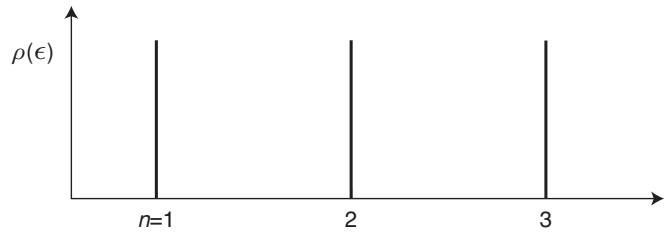
\includegraphics[width=0.50\textwidth]{figs/ch15/fig_15.3_a.jpg}\\[4pt]
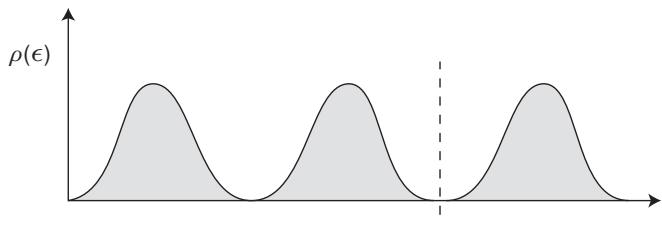
\includegraphics[width=0.50\textwidth]{figs/ch15/fig_15.3_b.jpg}
\caption*{图 15.3\quad (a) 磁场中朗道能级的态密度。(b) 无序导致的朗道能级展宽。虚线标示费米能的位置。}\label{fig:auto:15.3}
\end{figure}

从“扩展态只在每个朗道能级的中心形成而所有其他态都是局域的”这一简单图像出发，我们可以解释量子霍尔平台的起源。由于电流仅由每个朗道能级中心的态携带，当费米能扫过每个朗道能级的中心时，电流应当不连续地跳变。此外，若扩展态的占据保持不变，电流应保持恒定。也就是说，虽然增大磁场使化学势移离扩展态所在的神奇位置，但电导并不改变，因为此时化学势处于态被局域的区域。平台对应于扩展态中的粒子数固定的磁场范围。霍尔电压中出现严格平坦的台阶，证明了朗道能级中除中心处狭窄的扩展态区域之外所有态的极端局域化。正是由于这个原因，量子霍尔效应从根本上植根于无序。矛盾的是，无序并不影响霍尔电导的数值。具体地，青木（Aoki）和安藤（Ando）（AA1981）以及普兰格（Prange）（P1981; P1987）在漂移速度 $v_{x}=cE_{x}/B_{z}$ 的最低阶上证明：尽管一个孤立的 $\delta$ 函数杂质会束缚一个电子态，扩展态恰好携带足够的额外电流来补偿这一损失。

\section{边缘电流}

至此，我们论证了无序使所有电子态局域化，只有每个朗道能级未微扰能量附近窄窗内的态除外。一旦化学势移入这个区域，继续增大场对电导不再有影响，因为所有其他态都是局域的。于是，量子霍尔平台起源于扩展态与局域态之间的能量分隔。对完全平坦平台的可能偏离，或许仅来自从局域态到朗道能级中心处扩展态的热激活输运。在低温下，这类过程对输运的贡献可以忽略。

然而，我们还没有解释：为什么电导以 $e^{2}/h$ 整数倍的量子化如此精确。正如劳夫林（L1980）所指出的，电导的精确量子化暗示量子霍尔效应必定源于一条不带有任何材料参数（例如几何形状）的基本原理。为此，劳夫林表述了一个规范原理来解释霍尔电导的量子化。

为理解这一论证的要点，我们先就磁场中二维系统的电流作一个一般性的观察。如前所述，磁场中的电子因洛伦兹力而做圆周运动。如图 15.4 所示，在样品体内，相邻回旋轨道的顺时针与逆时针部分相互重叠，导致体内电流消失。然而在样品边缘，情况截然不同。在边缘处，轨道因边界产生的束缚势而被截断。电子一旦被边界反射，它仍试图做圆周运动。这就诱发了电子在样品边界上的跳跃式（skipping）运动，如图 15.4 所示。这种运动产生边缘电流，当磁场沿正 $z$ 方向取向时，电流沿顺时针方向流动。于是边缘电流的手性由磁场的方向决定。虽然上述论证严格成立的条件是磁性长度远大于电子的波长，即 $\ell\gg\hbar/p_{\mathrm{F}}$，但边缘电流的手性可以相当普遍地从边界处感应场的存在确立（W1990）。电流源自边缘处的态，这是量子霍尔系统一个真正新颖的特征。边缘电流的手性也是边缘态保持扩展的核心原因。正如我们在第 12 章中学到的，背散射对局域化的产生至关重要。手性边缘态不可能发生背散射。因此它们抵抗无规势引起的局域化。

\begin{figure}[H]\centering
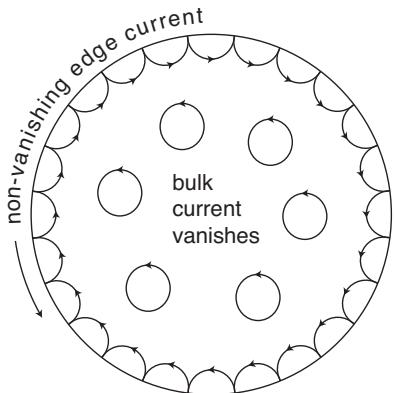
\includegraphics[width=0.46\textwidth]{figs/ch15/fig_15.4.jpg}
\caption*{图 15.4\quad 量子霍尔系统中的回旋轨道。圆轨道由洛伦兹力引起。在样品体内，回旋轨道的顺时针与逆时针部分重叠相消，导致体内电流消失。在边缘处，轨道被截断，产生边缘电流。}\label{fig:auto:15.4}
\end{figure}

既然电流完全由边缘携带，系统的几何形状便无关紧要。这一简单的认识已经暗示：量子霍尔效应中的电流是一个拓扑不变量。于是我们考虑一个中心挖孔的量子霍尔圆盘，如图 15.5 所示。这一几何与霍尔珀林（Halperin）（H1982）在重新表述原始劳夫林论证时所用的几何等价。圆盘被沿正 $z$ 方向的均匀磁场穿过。回旋轨道在圆盘外缘的截断导致沿顺时针方向流动的边缘电流。而在内半径处，束缚导致沿相反方向的电流。于是显然，若圆环的内外边缘处于同一化学势，系统中将没有净电流流动。让我们假设内外边缘的费米能级相差 $eE_{0}$。这个差别可能来自内外边缘束缚势的不对称，也可能来自可能存在的任何电化学势。若 $n$ 个朗道能级被占据，则总电势降为 $neE_{0}$。现在可以援引导出式 (15.23) 的同一论证，立即得到内外边缘之间的净电流以 $e^{2}/h$ 为单位量子化。

不过，只需稍加努力，我们便能以另一种方式得到同样的结果。现在考虑图 15.5(b) 所示的第二种几何。在表述规范论证时，我们会发现采用这一几何更为容易，因为前面使用的朗道规范可直接适用。我们的坐标系选成使 $y$ 坐标沿丝带环绕。与前一样，电流仅由边缘态携带。这些态环绕丝带一周并在回到原点时保持相位相干。为使刻画边缘态的波函数为单值，绕盘一周所包围的通量必须是 $2\pi$ 的整数倍。因此，我们对矢势所做的任何改变都应满足条件
\begin{equation*}
A=\frac{nhc}{eL},\tag{15.26}
\end{equation*}
其中 $L$ 是丝带的周长。对矢势的小改变，系统中的电流是规范不变的。现在考虑某个单粒子态 $\Psi_{\alpha}$ 的能量
\begin{equation*}
\epsilon_{\alpha}=\langle\Psi_{\alpha}|H|\Psi_{\alpha}\rangle\tag{15.27}
\end{equation*}
其中 $H$ 由式 (15.11) 的左端给出。为记号简便，我们定义 $\alpha=(n,k)$。我们关心的是 $\epsilon_{\alpha}$ 对 $A$ 的导数。为简化这个导数，我们利用黑尔曼--费曼（Hellman--Feynman）定理（H1937）
\begin{equation*}
\frac{\partial E(\lambda)}{\partial\lambda}=\langle\Psi_{\alpha}|\frac{\partial H(\lambda)}{\partial\lambda}|\Psi_{\alpha}\rangle,\tag{15.28}
\end{equation*}
其中 $\lambda$ 只是哈密顿量中的某个变量。将单粒子能量对 $A$ 求变分，
\begin{align*}
\frac{\partial\epsilon_{\alpha}}{\partial A}&=\frac{-e}{mc}\langle\Psi_{\alpha}|\mathbf{p}-\frac{eA}{c}|\Psi_{\alpha}\rangle\\
&=L\frac{I_{\alpha}}{c},\tag{15.29}
\end{align*}
便定义了态 $\alpha$ 掠过圆盘时携带的电流密度。为计算该导数，我们注意到，在电场存在时，单粒子能量随 $eE_{0}x_{k}$ 线性变化，其中 $x_{k}$ 标出组成每个朗道能级的态的中心。若我们修改哈密顿量中的规范项，使 $\mathbf{A}=Bx\widehat{y}\rightarrow Bx\widehat{y}+\Delta A\widehat{y}$，则每个中心的位置移动 $x_{k}\rightarrow x_{k}-\Delta A/B$。于是单粒子能量平移为 $\epsilon_{n,k}\rightarrow\epsilon_{n,k}-eE_{0}\Delta A/B$，且
\begin{equation*}
\frac{\partial\epsilon_{\alpha}}{\partial A}=-\frac{eE_{0}}{B}\tag{15.30}
\end{equation*}
与态指标无关。如图 15.6 所示，劳夫林规范原理（L1980）来自这样一个事实：同一朗道能级中相邻两态中心位置之差
\begin{align*}
\Delta x_{k}&=x_{k}^{m+1}-x_{k}^{m}=\ell^{2}(k_{m+1}-k_{m})=\frac{2\pi\ell^{2}}{L}\\
&=\frac{hc}{eBL}=\frac{\Delta A}{B},\tag{15.31}
\end{align*}
与矢势的改变直接相关。因此，若 $A$ 改变一个磁通量子，第 $m$ 个中心的位置
\begin{equation*}
x_{k}^{m}\rightarrow x_{k}^{m}-\frac{\Delta A}{B}=x_{k}^{m}-\frac{hc}{eBL}=x_{k}^{m-1}\tag{15.32}
\end{equation*}
就与第 $m-1$ 个中心的位置重合。于是，当一个磁通量子穿过丝带时，朗道能级中的态整体移动一个位置，导致（每个朗道能级）一个电子从样品的一边净转移到另一边。规范的量子化导致电荷转移的量子化！这就是劳夫林规范原理。它漂亮地阐明了量子霍尔效应中电荷输运的拓扑性质（T1982）。为计算电流，我们把式 (15.30) 代入式 (15.29)，并对所有被占据的朗道能级求和。立即得到两边缘之间的净电流
\begin{align*}
I&=\sum_{n,k}I_{n,k}\\
&=-\frac{ecN_{\mathrm{e}}E_{0}}{LB}=-\frac{ecnn_{B}V_{\mathrm{H}}}{B}=-\frac{ne^{2}V_{\mathrm{H}}}{h},\tag{15.33}
\end{align*}
它是 $e^{2}/h$ 的整数倍，其中 $V_{\mathrm{H}}=E_{0}W$ 为霍尔电压，$N_{\mathrm{e}}=nn_{B}LW$。电流中的负号对应于丝带上逆时针的运动。劳夫林的论证清楚地揭示：霍尔电流或霍尔电导的量子化主要来自扩展态沿样品边缘行进时必须单值的这一限制。对磁场中的系统而言，本征态的单值性表现为对容许规范变换的一个条件。正是这个条件加上朗道能级的整数填充导致了量子化。同样至关重要的是，规范变换必须绝热地实施，使得在穿透系统的磁通改变时系统仍停留在其基态。

\begin{figure}[H]\centering
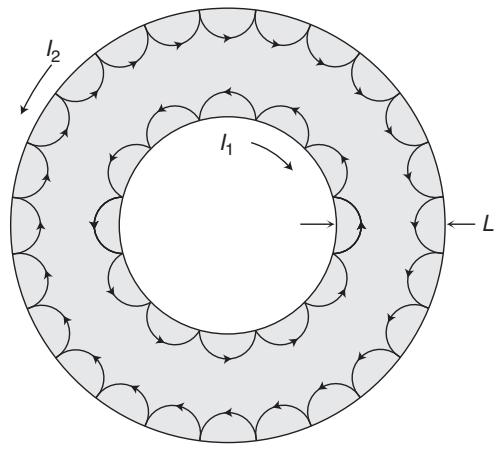
\includegraphics[width=0.50\textwidth]{figs/ch15/fig_15.5_a.jpg}\\[6pt]
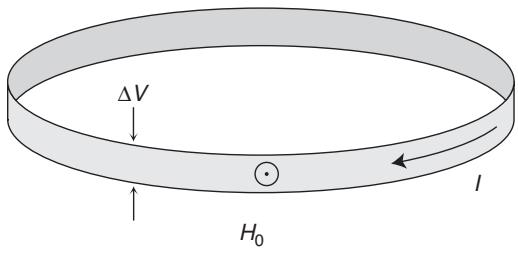
\includegraphics[width=0.62\textwidth]{figs/ch15/fig_15.5_b.jpg}
\caption*{图 15.5\quad (a) 被垂直纸面向外的磁场穿过的量子霍尔圆盘。箭头指示边缘电流的方向。(b) 磁场处处垂直于表面的量子霍尔丝带。这一几何在数学上等价于一个方向具有周期边界条件的矩形。丝带的周长为 $L$，宽度为 $W$。霍尔电压为 $\Delta V=E_{0}W$。}\label{fig:auto:15.5}
\end{figure}

\begin{figure}[H]\centering
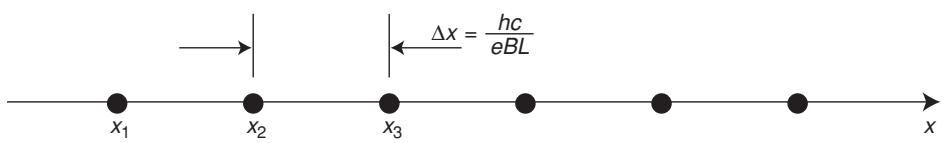
\includegraphics[width=0.72\textwidth]{figs/ch15/fig_15.6.jpg}
\caption*{图 15.6\quad 组成每个朗道能级的电子态中心的位置。所有态都被假定为简并的，其中心由 $\ell^{2}k_{m}=2\pi\hbar cm/eBL$ 给出。两中心之差为 $hc/eBL$。让一个磁通量子穿过样品，便把第 $m$ 个态变成第 $m-1$ 个，导致电荷从样品一边向另一边的转移。}\label{fig:auto:15.6}
\end{figure}

由于平台转变由磁场或填充的改变驱动，它们构成前一章所研究的那类真正的量子相变。事实上，由于无序是整数量子霍尔效应故事的核心，其背后的平台转变代表了无序系统中量子临界现象最清晰的实例之一。在理解平台转变的背后场论描述方面的进展，主要基于 Chalker--Coddington 隧穿网络模型（CC1988; MT1999; Z1999）。对该模型的数值模拟（LWK1993; LC1994）给出关联长度指数 $\nu=2.3$，与实验观察一致。然而，这一指数尚未由严格的理论推演所预言。

\section{拓扑绝缘体}

在量子霍尔效应中，电流由边缘携带。电流必须是 $e^{2}/h$ 的整数倍，这完全由如下事实决定：当电磁规范改变一个磁通量子时，有一个电荷被输运穿过样品。由于边缘态必须单值，而其单值性对电磁规范的可能改变施加了约束，量子霍尔系统中的电流是稳固的。样品的拓扑是唯一的决定因素，因为 $\sigma_{xy}$ 完全是边缘效应。虽然样品的边缘导电，体内却完全绝缘。因此，量子霍尔样品是拓扑绝缘体。由于时间反演对称性被破坏，正向与反向运动的边缘态在空间上是分离的。因此，若画出量子霍尔系统近边缘处的能带结构，它看起来会像图 15.7 那样。图中画出两个朗道能级之间的带隙以及一条穿越带隙的边缘态。量子霍尔系统中的关键观察是 $2=1+1$。也就是说，共有两个边缘态，但由于时间反演对称性的破坏，每个边缘只有一个。如前所指出的，每个边缘上杂质引起的弹性散射不会导致背散射，因为每个边缘上的态只沿单一方向传播。存在这样的可能性：来自一个边缘的弹性散射产生一个反向传播的态。但这将要求一个电子跃过样品跳到另一边缘。然而这种事件的概率是指数地小的。因此，电子遇到弹性杂质时唯一的选择就是绕过它并继续沿原方向运动。

\begin{figure}[H]\centering
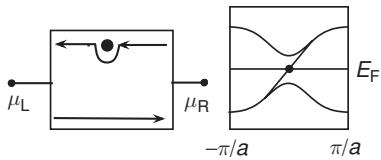
\includegraphics[width=0.42\textwidth]{figs/ch15/fig_15.7.jpg}
\caption*{图 15.7\quad (a) 具有手性边缘态的量子霍尔条。(b) 相应的量子霍尔系统示意能带结构，单一边缘态穿越带隙。在不存在时间反演对称性破坏时，特定手性的边缘态穿越费米能级一次。}\label{fig:auto:15.7}
\end{figure}

现在考虑关掉磁场。是否仍可能有对背散射免疫的边缘态？答案是肯定的。正是这一简单的认识催生了拓扑绝缘体领域（KM2005a; KM2005b; TFK2008; HK2010; BHZ2006; R2009; MB2007; X2009; Z2009; QHZ2008; QZ2010; K2007; BZ2006）。这里的关键是 $4=2+2$（QZ2010）。也就是说，当时间反演对称性保持时，每个边缘必须有两个传播态。每个边缘处的时间反演对称性保证正向与反向传播态具有相反的自旋。当然，若电子散射到样品的另一侧，它可以向相反方向运动。这里同样，这是一个指数地小的过程。因此，只要杂质是无结构的，即由杂质产生的相互作用不能混合自旋，就没有办法背散射电子。然而，如上表述的这个论证在自旋--轨道散射存在时会失效。拯救我们的是自旋-$1/2$ 粒子时间反演的一个非凡性质。在量子力学中，自旋-$1/2$ 粒子的时间反演算符由反幺正算符
\begin{equation*}
T=\mathrm{e}^{\mathrm{i}\frac{\pi}{2}\sigma_{y}}K\tag{15.34}
\end{equation*}
支配，其中 $\sigma_{y}$ 是第 7 章定义的 $y$ 泡利矩阵，$K$ 执行复共轭。利用 $\sigma_{y}^{2}=1$ 这一事实，可以展开时间反演算符中的指数

\begin{figure}[H]\centering
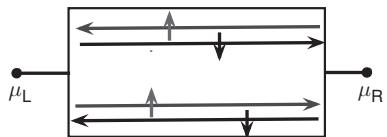
\includegraphics[width=0.46\textwidth]{figs/ch15/fig_15.8.jpg}
\caption*{图 15.8\quad 每个边缘具有两个传播态的量子自旋霍尔系统。克拉默斯定理意味着这样的态必定双重简并。上下箭头标示自旋。}\label{fig:auto:15.8}
\end{figure}

并确立：对任意角 $\alpha$，
\begin{equation*}
\mathrm{e}^{\mathrm{i}\alpha\sigma_{y}/2}=\mathrm{i}\alpha\sigma_{y}\sin\alpha/2+\cos\alpha/2.\tag{15.35}
\end{equation*}
因此，把自旋-$1/2$ 粒子旋转 $2\pi$ 并不使粒子回到原来的态，而是回到其负号，且 $T^{2}=-1$。这就是克拉默斯倍增（Kramers doubling）的起源。即：时间反演不变（TRI）哈密顿量的所有本征态必定双重简并。因此，边缘态必须成对出现，每个自旋一个，如图 15.8 所示。

$T^{2}=-1$ 在自旋--轨道散射存在时保护表面态不打开能隙，这可以用两种方式之一说明。先考虑弹性散射的后果。在半经典图像中，一个正向运动的电子遇到一个可以有自旋--轨道散射的杂质时，可能被反射回去。然而，由于所论边缘上反向运动的唯一通道具有相反的自旋，电子必须翻转其自旋。在此过程中，自旋获得相位 $\pi$。将此过程沿时间反演，TRI 意味着存在一个等价过程：正向运动的电子被散射回去，但获得相位变化 $-\pi$。（这两个过程可以想作自旋的逆时针与顺时针旋转。）只要 TRI 存在，这两个振幅的大小就相同。然而这两条路径之间的相位变化是 $2\pi$，故波函数改变 $-1$。两条路径相加给出为零的杂质散射振幅；也就是说，存在完全的相消干涉。因此，只要 TRI 存在，就没有办法从杂质上背散射，表面态必然穿越能隙，从而产生净的纵向电流。或者，我们可以从能带论证确立表面态的稳固性。TRI 意味着表面态必须以相等相反的动量成对出现。把哪个动量指定为自旋向上或向下是无关紧要的。此外，在布里渊区中的 TRI 点处，边缘态必须具有相同的能量，对一维边缘态这些点是 $k=0$ 与 $k=\pi/a$。注意，$k=-\pi/a$ 点按 TRI 与 $\pi/a$ 等同。在远离 TRI 点处，自旋--轨道相互作用可以解除边缘态之间的简并。问题是简并如何被解除。若这对边缘态像图 15.9(a) 那样连接两个简并点，则表面态并不稳固。图 15.9(a) 与图 15.9(b) 拓扑上等同，因为化学势可以在带隙中上下移动。注意，边缘态穿越费米能两次这件事无关紧要。只要它们穿越偶数次，总能构造出与图 15.9(b) 类似的情形。于是边缘态获得质量。然而这并非唯一的选择。简并也可以这样被解除：在远离 TRI 点处只有一个单一的穿越，如图 15.9(c) 所示。在这种情况下，样品无法以任何方式被变形（例如切割）以消除这个单一穿越点。也就是说，这样的态受到拓扑保护。我们可以通过定义指标（TFK2008; KM2005a; KM2005b）
\begin{equation*}
N_{\mathrm{K}}=m\ \mathrm{mod}\ 2,\tag{15.36}
\end{equation*}
来区分这两种情形，其中 $N_{\mathrm{K}}$ 是穿越费米能的边缘态克拉默斯对的数目。为明确起见，$m\ \mathrm{mod}\ 2$ 只是指 $m+2p$，其中 $p$ 为任意整数。若 $N_{\mathrm{K}}$ 为偶，则 $m=0$；而 $m=1$ 对应 $N_{\mathrm{K}}$ 为奇。由于 $m$ 只有两个可能的取值，我们可以把 $m$ 看作一个 $Z_{2}$ 不变量。$Z_{2}$ 是具有两个元素的群，即 1 与 0，因而是最简单的非平凡群。

\begin{figure}[H]\centering
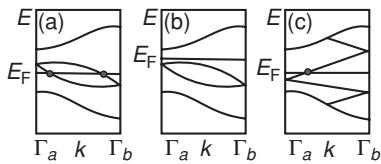
\includegraphics[width=0.46\textwidth]{figs/ch15/fig_15.9.jpg}
\caption*{图 15.9\quad 两个克拉默斯简并（或时间反演不变）点 $\Gamma_{a}$ 与 $\Gamma_{b}$ 之间的电子色散。对二维样品，简并点位于 $\Gamma_{a}=0$ 与 $\Gamma_{b}=\pi/a$。(a) 费米穿越点数目为偶数时，表面态在两个克拉默斯点之间的演化。(b) (a) 的一个变形，它在表面态中打开能隙。只要边缘态穿越化学势偶数次，(a) 的这样一种变形总是可能的。因此 (a) 与 (b) 拓扑上不可区分。在 (c) 中只有一个单一的穿越点，此时样品的任何变形都保持边缘态的完整性。}\label{fig:auto:15.9}
\end{figure}

这里有一些微妙的东西，通过考虑二维的自旋自由电子可以把它讲清楚。若时间反演对称性存在，对于在 (2+1) 维系统边缘上传播的电子，能写出的最简单哈密顿量是
\begin{equation*}
H=p\sigma^{z}.\tag{15.37}
\end{equation*}
我们问一个简单的问题：这样的边缘态如何才能打开能隙？最简单的增补是加上形如 $m_{\nu}\sigma^{y}+m_{z}\sigma^{z}$ 的项。然而，由于质量在 $t\rightarrow-t$ 下保持不变，这种耦合破坏 TRI，因而是不允许的。为打开能隙，我们需要考虑多于单对边缘态的情形。考虑系统的两个副本：
\begin{equation*}
H^{(2)}=p\mathbf{I}\otimes\sigma^{z}=\begin{pmatrix}p\sigma^{z} & 0\\ 0 & p\sigma^{z}\end{pmatrix}.
\end{equation*}
在这个扩大了的空间中，我们（在 TRI 存在下）可以通过添加形如 $m\tau^{y}\otimes\sigma^{x}$ 的项来产生能隙，使得
\begin{equation*}
H^{(2)}\rightarrow p\mathbf{I}\otimes\sigma^{z}+m\tau^{y}\otimes\sigma^{x}\tag{15.38}
\end{equation*}
其中
\begin{equation*}
\tau^{y}=\begin{pmatrix}0 & -\mathrm{i}\\ \mathrm{i} & 0\end{pmatrix}.
\end{equation*}
这个矩阵的本征值
\begin{equation*}
\lambda_{\pm}=\pm\sqrt{p^{2}+m^{2}},\tag{15.39}
\end{equation*}
双重简并且具有能隙。因此，除非存在单个狄拉克锥（或奇数个狄拉克锥），边缘态都容易打开能隙。

虽然这些物理可以推广到三维样品的边缘，在四个空间维度中有这类物理的一个更熟悉的场所，即手性费米子。这样的费米子描述 (4+1) 维系统边界上的传播模式。边界态由两个外尔（而非狄拉克）方程描述：
\begin{equation*}
\left(\boldsymbol{\sigma}\cdot\nabla-\mathrm{i}\frac{\partial}{\partial x_{0}}\right)\phi^{(\mathrm{L})}=0,\quad\left(-\boldsymbol{\sigma}\cdot\nabla-\mathrm{i}\frac{\partial}{\partial x_{0}}\right)\phi^{(\mathrm{R})}=0,\tag{15.40}
\end{equation*}
其中 $x_{0}=t$。在这些方程中我们为简单起见已取 $\hbar=c=1$。然而，这并不是两个手性费米子最一般的描述。例如，其中没有质量项。让我们定义两分量旋量
\begin{equation*}
\psi=\begin{pmatrix}\phi^{(\mathrm{R})}\\ \phi^{(\mathrm{L})}\end{pmatrix}.\tag{15.41}
\end{equation*}
解耦外尔方程的有质量推广
\begin{equation*}
\left(\mathrm{i}\gamma_{\mu}\partial_{\mu}-m\right)\psi=0,\tag{15.42}
\end{equation*}
是狄拉克方程，$\gamma_{\mu}$ 为狄拉克矩阵。让我们定义 $\sigma^{\mu}=(I,\boldsymbol{\sigma})$，即 $\sigma^{0}=I$。由这一矩阵运动方程分量的形式
\begin{equation*}
\begin{pmatrix}\mathrm{i}\sigma^{\mu}\cdot\partial_{\mu} & -m\\ -m & \mathrm{i}\sigma^{\mu}\cdot\partial_{\mu}\end{pmatrix}\begin{pmatrix}\phi^{(\mathrm{R})}\\ \phi^{(\mathrm{L})}\end{pmatrix}=0,\tag{15.43}
\end{equation*}
显而易见，质量项使左移与右移者耦合。因此，只有当左移与右移对都像图 15.9(b) 中那样穿越化学势时，它们才能被耦合并产生质量。更精确地说，左移与右移者的每个外尔方程各有其自己的 SU(2) 对称性。因此总对称性为 $\mathrm{SU}(2)\times\mathrm{SU}(2)$。非零质量意味着波函数的左、右分量不能独立转动。也就是说，对称性已降低为一个整体 SU(2)。

什么类型的哈密顿量导致拓扑绝缘？通常它们涉及自旋--轨道相互作用。考虑一个简单模型（BHZ2006）：
\begin{align*}
H=\sum_{m,n}\frac{1}{2}\Big[&\Psi_{m+1,n}^{\dagger}(\mathrm{i}\Gamma^{x}-\Gamma^{0})\Psi_{m,n}+\Psi_{m,n}^{\dagger}(-\mathrm{i}\Gamma^{x}-\Gamma^{0})\Psi_{m+1,n}\\
&+\Psi_{m,n+1}^{\dagger}(\mathrm{i}\Gamma^{y}-\Gamma^{0})\Psi_{m,n}+\Psi_{m,n}^{\dagger}(-\mathrm{i}\Gamma^{y}-\Gamma^{0})\Psi_{m,n+1}\Big]+(2-M)\Psi_{m,n}^{\dagger}\Gamma^{0}\Psi_{m,n}\tag{15.44}
\end{align*}
每个格点有两个轨道，且具有最近邻跳跃。这里
\begin{equation*}
\Psi_{m,n}=(c_{\uparrow A},\,c_{\uparrow B},\,c_{\downarrow A},\,c_{\downarrow B})_{m,n}^{\mathrm{T}}\tag{15.45}
\end{equation*}
是对应于双轨道基组的旋量，且 $\Gamma^{x}=\sigma^{z}\otimes\tau^{x}$，$\Gamma^{y}=\mathbf{I}\otimes\tau^{y}$，$\Gamma^{0}=\mathbf{I}\otimes\tau^{z}$。这里 $\tau^{a}$ 是轨道基组中的泡利矩阵，$\sigma^{a}$ 是自旋基组中的泡利矩阵。这个哈密顿量被带到对角形式
\begin{equation*}
H=\sum_{\mathbf{k}}H(\mathbf{k})\Psi^{\dagger}(\mathbf{k})\Psi(\mathbf{k}),\tag{15.46}
\end{equation*}
所用的傅里叶变换为
\begin{equation*}
\Psi(\mathbf{k})=\frac{1}{\sqrt{N}}\sum_{m,n}\mathrm{e}^{\mathrm{i}(k_{x}m+k_{y}n)}\Psi_{m,n}.\tag{15.47}
\end{equation*}
$4\times4$ 的布洛赫哈密顿量为
\begin{equation*}
H(\mathbf{k})=\Gamma^{x}\sin k_{x}+\Gamma^{y}\sin k_{y}+\Gamma^{0}(2-M-\cos k_{x}-\cos k_{y}).\tag{15.48}
\end{equation*}
对这个 $4\times4$ 哈密顿量，
\begin{equation*}
T=\mathrm{i}\sigma^{y}\otimes\mathbf{I}\,K\tag{15.49}
\end{equation*}
是时间反演算符。矩阵 $\Gamma^{x}$ 与 $\Gamma^{y}$ 在时间反演下均为奇，而 $\Gamma^{0}$ 为偶。由于前者与 $\sin k_{i}$ 耦合、后者与 $\cos k_{i}$ 耦合，哈密顿量是 TRI 的。虽然这个哈密顿量是 $4\times4$ 的，它由 $2\times2$（自旋）块组成，每块形如
\begin{equation*}
H_{\mathrm{LD}}=d_{a}(\mathbf{p})\tau^{a},\tag{15.50}
\end{equation*}
其中 $d_{a}(\mathbf{p})$ 是一个三分量矢量，其第三个分量是质量项。写成这种形式便可清楚地看到，每个自旋扇区中的质量项决定时间之箭的方向，因为它在时间反演下为奇。十分普遍地，所有拓扑绝缘体模型都可以约化为这种形式的某种东西。对角化后，我们求得哈密顿量的本征值为
\begin{equation*}
E_{\pm}=\pm\sqrt{\sin^{2}k_{x}+\sin^{2}k_{y}+M^{2}(\mathbf{k})},\tag{15.51}
\end{equation*}
其中 $M(\mathbf{k})=2-M-\cos k_{x}-\cos k_{y}$。这一色散对应于有质量外尔方程的两个副本，每个自旋一个，$M$ 为质量。在长波极限下，$E_{\pm}(\mathbf{k}\rightarrow0)\rightarrow\pm\sqrt{k_{x}^{2}+k_{y}^{2}+M^{2}}$。质量在特殊的 $M$ 值处消失。例如在 $M=0,2,4$ 时，谱分别在 (1) $(0,0)$、(2) $(\pi,0)$ 与 $(0,\pi)$、以及 (3) $(\pi,\pi)$ 处无隙。由于这些是布里渊区中决定低能物理的仅有的点，我们把哈密顿量在每个这样的动量附近展开：
\begin{align*}
H_{\uparrow}(k_{x}=0,\,k_{y}=0)&=k_{x}\tau^{x}+k_{y}\tau^{y}-M\tau^{z},\tag{15.52}\\
H_{\uparrow}(k_{x}=\pi,\,k_{y}=0)&=-k_{x}\tau^{x}+k_{y}\tau^{y}+(2-M)\tau^{z},\tag{15.53}\\
H_{\uparrow}(k_{x}=0,\,k_{y}=\pi)&=k_{x}\tau^{x}-k_{y}\tau^{y}+(2-M)\tau^{z},\tag{15.54}\\
H_{\uparrow}(k_{x}=\pi,\,k_{y}=\pi)&=-k_{x}\tau^{x}-k_{y}\tau^{y}+(4-M)\tau^{z},\tag{15.55}
\end{align*}
（译注：式 (15.53) 原文括号内第二处印作 $k_{x}=0$，按本意应为 $k_{y}=0$。）对给定的自旋，比如说 $\uparrow$。$\downarrow$ 自旋扇区的方程由 $H(\mathbf{k})$ 的下对角块构造，它只是改变 $k_{x}$ 项的符号。

我们想确定这些边缘态中的每一个对霍尔电导的贡献。哈密顿量的每个 $2\times2$ 块描述单个狄拉克锥（Dirac cone），所以我们需要计算单个狄拉克锥的霍尔电导。这可以用如下对称性论证完成。考虑在一个具有单狄拉克锥的哈密顿量中分隔质量正负号的畴壁（domain wall），如图 15.10 所示。在 $m=0$ 的畴壁处局域着一个单一的边缘模式。因此，按我们先前的讨论，边缘态携带的电导为 $e^{2}/h$。由对称性，系统两侧对边缘电流的贡献必须相等。于是每个狄拉克锥的电导必为电导量子的一半。此外，电导的正负号由狄拉克方程中质量项的正负号决定。从图 15.10 可以这样理解：边缘模式位于负质量区域的右侧，却位于正质量区域的左侧。因此每个区域诱发的电流方向取决于该区域中质量的正负号。在一般情形下，这个正负号由轨道“自旋”$(\tau^{x},\tau^{y},\tau^{z})$ 围绕狄拉克锥的排布方式决定，图 15.10 中的箭头示出了这种排布。所以，式 (15.50) 中动量的正负号也对霍尔电导的正负号有贡献。这也可以从下面的方式看出。在二维，宇称算符
\begin{equation*}
P(x,y)\rightarrow(-x,y)\quad\text{或}\quad(x,-y)\tag{15.56}
\end{equation*}
只作用于一个坐标。因此，令 $k_{x}\rightarrow-k_{x}$ 会翻转霍尔电导的正负号。

\begin{figure}[H]\centering
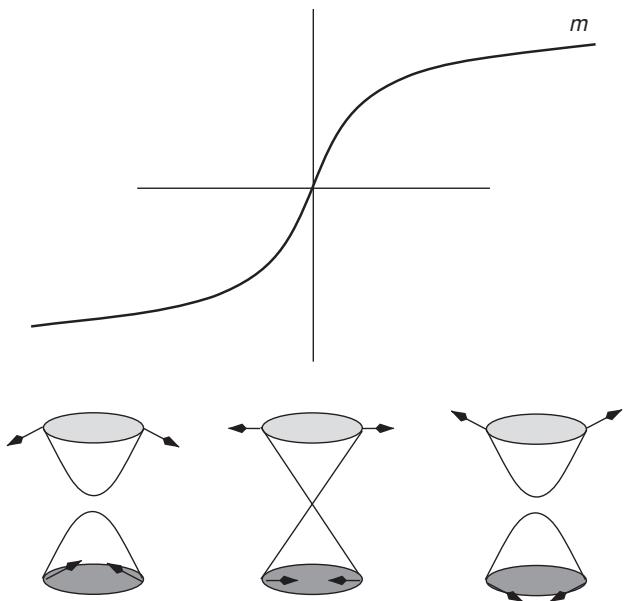
\includegraphics[width=0.55\textwidth]{figs/ch15/fig_15.10.jpg}
\caption*{图 15.10\quad 狄拉克哈密顿量质量中的畴壁。图中示意地画出每个质量取值处态的谱。箭头显示给定 $k$ 处轨道“自旋”$(\tau^{x},\tau^{y},\tau^{z})$ 的期望值。由于边缘处的电导为 $e^{2}/h$ 且仅来自狄拉克锥，每个锥的电导为 $e^{2}/2h$。}\label{fig:auto:15.10}
\end{figure}

为确定每个狄拉克点处电导的实际数值，我们采用如下约定：若相应的哈密顿量形如 $k_{x}\sigma^{x}+k_{y}\sigma^{y}+M\sigma^{z}$，则电导为 $(e^{2}/2h)\,\mathrm{sgn}(M)$。考虑 $M<0$ 时 $(0,0)$ 点的哈密顿量。它恰是给出电导 $e^{2}/2h$ 的形式。现在考虑 $(\pi,0)$ 点。与 $(0,0)$ 点相比，需令 $k_{x}\rightarrow-k_{x}$，于是 $(\pi,0)$ 点给出贡献 $-e^{2}/2h$。在 $(0,\pi)$ 点（译注：原文此处印作 $(\pi,0)$ 点），必须令 $k_{y}\rightarrow-k_{y}$ 才能恢复所需的形式，故电导为 $-e^{2}/2h$。在 $(\pi,\pi)$ 点则需要两次正负号改变，因而为 $e^{2}/2h$。所有这些之和为零。因此，对 $M<0$，无论自旋 $\uparrow$ 还是自旋 $\downarrow$，表面都没有净导电，得到的是平凡绝缘体。同样的分析可用于 $0<M<2$、$2<M<4$ 与 $M>4$。结果示于表 15.1。

\begin{center}
\small
表 15.1\quad 在式 (15.48) 所定义的模型中，对边缘输运有贡献的每个狄拉克锥的霍尔电导。霍尔电导以 $e^{2}/h$ 为单位，$M$ 为质量。表中同时给出每个自旋的总霍尔电导 $\sigma_{xy,\uparrow}$、净霍尔电导 $\sigma_{xy}$ 以及自旋霍尔电导 $\sigma_{xy}^{\mathrm{s}}$。

\vspace{4pt}
\begin{tabular}{lcccc}
\toprule
$k$ & $M<0$ & $0<M<2$ & $2<M<4$ & $M>4$ \\
\midrule
$(0,0)$ & $1/2$ & $-1/2$ & $-1/2$ & $-1/2$ \\
$(\pi,0)$ & $-1/2$ & $-1/2$ & $1/2$ & $1/2$ \\
$(0,\pi)$ & $-1/2$ & $-1/2$ & $1/2$ & $1/2$ \\
$(\pi,\pi)$ & $1/2$ & $1/2$ & $1/2$ & $-1/2$ \\
\midrule
$\sigma_{xy,\uparrow}$ & $0$ & $-1$ & $1$ & $0$ \\
$\sigma_{xy,\downarrow}$ & $0$ & $+1$ & $-1$ & $0$ \\
$\sigma_{xy}$ & $0$ & $0$ & $0$ & $0$ \\
$\sigma_{xy}^{\mathrm{s}}$ & $0$ & $-2$ & $+2$ & $0$ \\
\bottomrule
\end{tabular}
\end{center}

由于 $k_{x}$ 对自旋 $\downarrow$ 改变正负号，每个节点的霍尔电导对相反自旋的块改变正负号。因此，正如 TRI 所要求的，净霍尔电导总为零。但如果我们现在定义一个自旋霍尔电导（BZ2006; KM2005a）
\begin{equation*}
\sigma_{xy}^{\mathrm{s}}=\sum_{s=\uparrow,\downarrow}\mathrm{sgn}\left(s\right)\sigma_{xy,s}\tag{15.57}
\end{equation*}
我们发现，对 $0<M<2$，$\sigma_{xy}^{\mathrm{s}}=-2e^{2}/h$；对 $2<M<4$，则为 $2e^{2}/h$。对所有其他取值，它为零，得到平凡绝缘体。

在诸如 HgTe/HgCdTe 这样的量子阱系统中，$M$ 的数值只需通过改变量子阱的厚度来调节。特别地，当量子阱厚度超过一个临界值时，$M$ 的正负号可以改变。这首先由贝内维格（Bernevig）、休斯（Hughes）和张（Zhang）（BHZ2006）预言。为确认拓扑绝缘体的存在，已在 HgTe/HgCdTe 量子阱上完成了最先进的实验（K2007）。在图 15.8 的几何中，从左（L）到右（R）的电流由两个导电边缘模式携带，顶边与底边各占每个自旋的一个。于是，基于边缘图像，拓扑态中的电导必为 $G_{\mathrm{LR}}=2e^{2}/h$。这在实验中已被清楚地观察到，如图 15.11 所示。我们必须注意，虽然各自旋通道的电导相加，但这并不一定是拓扑绝缘体的稳固特征。只有在自旋通道不像式 (15.48) 中那样混合时，这种可加性才成立。

\begin{figure}[H]\centering
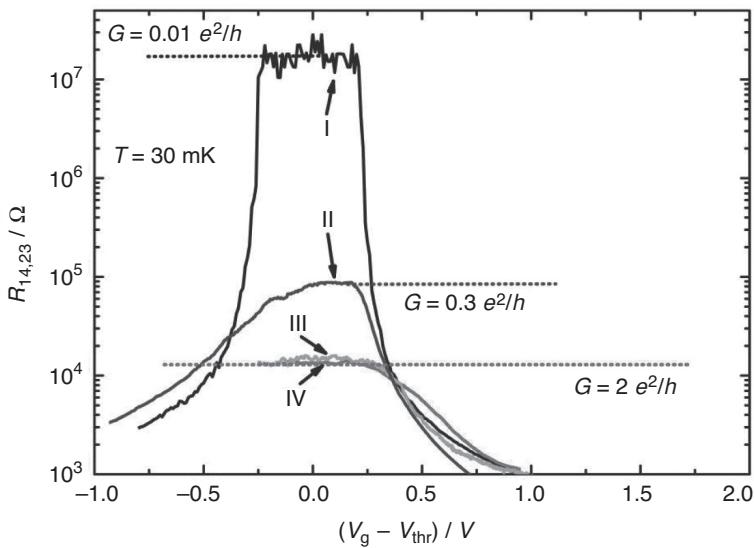
\includegraphics[width=0.55\textwidth]{figs/ch15/fig_15.11.jpg}
\caption*{图 15.11\quad 厚度低于（I）与高于（II、III、IV）临界值的各种量子阱系统的纵向电阻。系统 I 与 II（III 与 IV）的尺寸大于（小于）非弹性平均自由程。由于边缘处的非弹性背散射过程，系统 II 的电导未能达到预言值。图取自（K2007）。}\label{fig:auto:15.11}
\end{figure}

观察三维系统中表面模式的一个有力方法是角分辨光电子发射谱（ARPES），它能以精细的动量与能量分辨探测表面电子能带结构。候选材料已在 BiSb 合金以及 $\mathrm{Bi}_{2}\mathrm{Se}_{3}$ 和 $\mathrm{Bi}_{2}\mathrm{Te}_{3}$ 晶体中被确认（TFK2008; Z2009; X2009）。ARPES 测量证实了存在奇数个克拉默斯配对的表面模式（H2008; X2009; H2009）。图 15.12 给出 $\mathrm{Bi}_{2}\mathrm{Se}_{3}$ 的 ARPES 数据，它恰有一对这样的模式，在表面形成单个狄拉克锥。

\begin{figure}[H]\centering
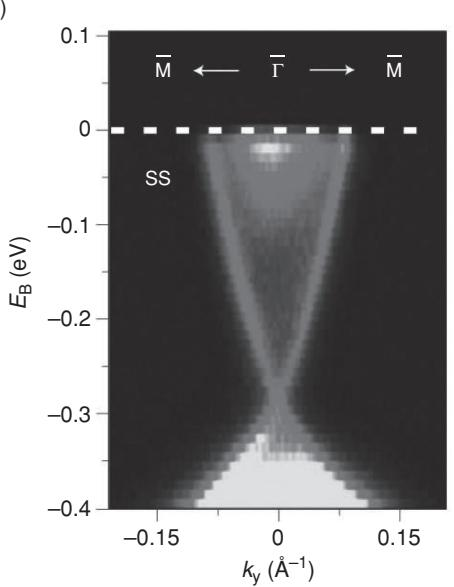
\includegraphics[width=0.46\textwidth]{figs/ch15/fig_15.12_a.jpg}\hfill
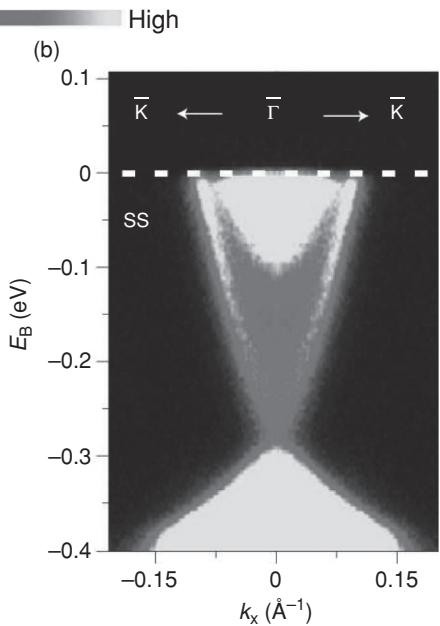
\includegraphics[width=0.46\textwidth]{figs/ch15/fig_15.12_b.jpg}
\caption*{图 15.12\quad $\mathrm{Bi}_{2}\mathrm{Se}_{3}$ 的 ARPES 数据显示，在体能隙之内，除体内（较浅灰色）的态以外，表面能带结构中存在单一的克拉默斯对。面板 a 与 b 显示动量空间中不同的切割。图取自（X2009）。}\label{fig:auto:15.12}
\end{figure}

\subsection{一般表述}

我们目前对拓扑绝缘体的表述完全建立在单粒子物理之上，并且相当特殊于两个空间维度。尽管如此，这些物理甚至在多粒子情形和三个空间维度中也成立。虽然可以把单粒子图像推进到 $d=3$（MB2007; R2009; HK2010），但这里我们采取另一种（QHZ2008; QZ2010）同样适用于多粒子的方法。固体中的相互作用电子对外电场和外磁场有明确清晰的响应。因此，我们把绝缘体的普遍作用量写成 $S=S_{0}+S_{\theta}$：其中总能量项为
\begin{equation*}
S_{0}=\frac{1}{8\pi}\int\mathrm{d}^{3}x\,\mathrm{d}t\left(\epsilon\mathbf{E}^{2}-\frac{1}{\mu}\mathbf{B}^{2}\right),\tag{15.58}
\end{equation*}
$\epsilon$ 与 $\mu$ 分别为介电常数与磁导率；另有附加项
\begin{equation*}
S_{\theta}=\left(\frac{\theta}{\pi c^{2}}\right)\left(\frac{e^{2}}{2h}\right)\int\mathrm{d}^{3}x\,\mathrm{d}t\,\mathbf{E}\cdot\mathbf{B},\tag{15.59}
\end{equation*}
它因为显然破坏时间反演对称性而通常被忽略。后一项描述磁电效应（magneto-electric effect）。然而，正如我们将看到的，当周期边界条件存在时，这一项是容许的。在显式计算这一项之前，我们先证明它完全约化为一个边界贡献，因而本质上是拓扑的。为简化 $S_{\theta}$ 项，我们回忆电磁场强度 $F_{\mu\nu}$ 通过
\begin{equation*}
F_{\mu\nu}\equiv\partial_{\mu}A_{\nu}-\partial_{\nu}A_{\mu},\tag{15.60}
\end{equation*}
与矢势相联系，其中
\begin{equation*}
A_{\mu}=(-\Phi,A^{1},A^{2},A^{3})\tag{15.61}
\end{equation*}
$\Phi$ 为标势。由于 $F_{\mu\nu}$ 是纯反对称的，对所有 $\mu$ 有 $F_{\mu\mu}=0$。定义 $i$ 为可取值 1、2 或 3 的空间指标，便得到
\begin{equation*}
F_{0i}=\frac{1}{c}\frac{\partial A^{i}}{\partial t}+\frac{\partial\Phi}{\partial x^{i}}=-E_{i}.\tag{15.62}
\end{equation*}
类似地，B 场的 $z$ 分量定义为
\begin{equation*}
F_{12}=\partial_{1}A_{2}-\partial_{2}A_{1}=\partial_{x}A_{y}-\partial_{y}A_{x}\equiv B_{z},\tag{15.63}
\end{equation*}
这当然等价于 $\mathbf{B}=\nabla\times\mathbf{A}$ 的 $z$ 分量。于是，电磁场强度具有分量
\begin{equation*}
F_{\mu\nu}=\left(\begin{array}{cccc}
0 & E_{x} & E_{y} & E_{z}\\
-E_{x} & 0 & B_{z} & -B_{y}\\
-E_{y} & -B_{z} & 0 & B_{x}\\
-E_{z} & B_{y} & -B_{x} & 0
\end{array}\right).\tag{15.64}
\end{equation*}
$\mathbf{E}$ 与 $\mathbf{B}$ 的点积于是约化为
\begin{equation*}
\mathbf{E}\cdot\mathbf{B}=F_{0i}F_{jk}\epsilon^{0ijk},\tag{15.65}
\end{equation*}
其中 $\epsilon^{0ijk}$ 是完全反对称张量。我们采用约定
\begin{equation*}
\epsilon^{0xyz}=1.\tag{15.66}
\end{equation*}
为得到 $S_{\theta}$ 实际上是一个拓扑项这一最终结果，我们引入一些简化记号。令
\begin{equation*}
F=\frac{1}{2}F_{\mu\nu}\,\mathrm{d}x^{\mu}\wedge\mathrm{d}x^{\nu},\tag{15.67}
\end{equation*}
其中
\begin{equation*}
\mathrm{d}x^{\mu}\wedge\mathrm{d}x^{\nu}=\mathrm{d}x^{\mu}\otimes\mathrm{d}x^{\nu}-\mathrm{d}x^{\nu}\otimes\mathrm{d}x^{\mu}.\tag{15.68}
\end{equation*}
一般地，对任意 1-形式（矢量上的线性算符）有 $v\wedge w=-w\wedge v$，故 $F$ 的定义中分母有因子 2。一般地，对 $n$-形式的反对称化，分母中出现 $n!$。因此
\begin{align*}
F\wedge F&=\frac{1}{4}F_{\mu\nu}F_{\rho\lambda}\,\mathrm{d}x^{\mu}\wedge\mathrm{d}x^{\nu}\wedge\mathrm{d}x^{\rho}\wedge\mathrm{d}x^{\lambda}\\
&=\frac{1}{4}\epsilon^{\mu\nu\rho\lambda}F_{\mu\nu}F_{\rho\lambda}\,\mathrm{d}x\wedge\mathrm{d}y\wedge\mathrm{d}z\wedge\mathrm{d}t,\tag{15.69}
\end{align*}
其中 $\mathrm{d}t\wedge\mathrm{d}x\wedge\mathrm{d}y\wedge\mathrm{d}z\equiv\mathrm{d}^{4}x$ 是四维体积元。利用这些定义与式 (15.65)，作用量中的附加项简化为
\begin{equation*}
S_{\theta}=\left(\frac{\theta}{\pi c^{2}}\right)\left(\frac{e^{2}}{2h}\right)\int\mathrm{d}^{3}x\,\mathrm{d}t\,\mathbf{E}\cdot\mathbf{B}=\left(\frac{\theta}{2\pi c^{2}}\right)\left(\frac{e^{2}}{2h}\right)\int F\wedge F.\tag{15.70}
\end{equation*}
用 1-形式的分量表示，$\mathbf{A}=A_{\mu}\mathrm{d}x^{\mu}$，
\begin{align*}
F&\equiv\mathrm{d}A=\partial_{\mu}A_{\nu}\,\mathrm{d}x^{\mu}\wedge\mathrm{d}x^{\nu}\\
&=\frac{1}{2}\left(\partial_{\mu}A_{\nu}-\partial_{\nu}A_{\mu}\right)\mathrm{d}x^{\mu}\wedge\mathrm{d}x^{\nu}\tag{15.71}
\end{align*}
因为 $F$ 是完全反对称的。注意 $F$ 是一个 2-形式，因为它包含两个微分。这使我们能把 $F\wedge F$ 简化为 $\mathrm{d}A\wedge\mathrm{d}A$。这种记法不只是一场练习。若我们分部积分，
\begin{equation*}
\int\mathrm{d}A\wedge\mathrm{d}A=\int\mathrm{d}(A\wedge\mathrm{d}A)+A\wedge\mathrm{d}^{2}A,\tag{15.72}
\end{equation*}
便生成一个含有算符 $\mathrm{d}^{2}A$ 的边界项。在得到这个结果时，我们使用了规则
\begin{equation*}
\mathrm{d}(A\wedge B)=\mathrm{d}A\wedge B+(-1)^{r}A\wedge\mathrm{d}B,\tag{15.73}
\end{equation*}
其中 $r$ 是形式的阶。式 (15.72) 之所以成立，是因为 $A$ 是 1-形式。由关于 $\mathrm{d}A$ 的规则（式 (15.71)），把该规则应用两次，便可立即写下 $\mathrm{d}^{2}A$ 的含义：
\begin{equation*}
\mathrm{d}^{2}A=\partial_{\lambda}\partial_{\mu}A_{\nu}\,\mathrm{d}x^{\lambda}\wedge\mathrm{d}x^{\mu}\wedge\mathrm{d}x^{\nu},\tag{15.74}
\end{equation*}
前面的两个导数是对称的，而后面的基 $\mathrm{d}x^{\lambda}\wedge\mathrm{d}x^{\mu}$ 是反对称的。因此 $\mathrm{d}^{2}A=0$。分部积分并注意到 $\mathrm{d}^{2}A=0$，我们把作用量中的拓扑项约化为
\begin{equation*}
S_{\theta}=\left(\frac{\theta}{\pi c^{2}}\right)\left(\frac{e^{2}}{2h}\right)\int\mathrm{d}(A\wedge\mathrm{d}A),\tag{15.75}
\end{equation*}
由斯托克斯（Stokes）定理，它进一步约化为一个边界积分
\begin{equation*}
S_{\theta}=\left(\frac{\theta}{\pi c^{2}}\right)\left(\frac{e^{2}}{2h}\right)\int_{\partial M}A\wedge\mathrm{d}A,\tag{15.76}
\end{equation*}
因此，作用量中的附加项完全是一个仅由拓扑决定的边界项。作为边界项，它不能改变运动方程。实际上，$S_{\theta}$ 就是第二陈数。

为把握 $S_{\theta}$ 中包含的内容，我们简化到一个特殊的规范选择，直接计算式 (15.59)。为简单起见，取 $A_{0}=0$，并选择 $\mathbf{B}=B_{z}\widehat{z}$，它给出 $\mathbf{E}=E_{z}\widehat{z}$。我们对 $S_{\theta}$ 的归一化现在将变得明朗。把这个规范选择代入式 (15.59) 得到
\begin{equation*}
S_{\theta}=\left(\frac{\theta}{\pi c^{2}}\right)\left(\frac{e^{2}}{2h}\right)\int\mathrm{d}\mathbf{a}\cdot\nabla\times\mathbf{A}\int\mathrm{d}t\,\mathrm{d}z\,\partial_{t}A^{z}.\tag{15.77}
\end{equation*}
假定所有维度在一个环面上都是周期的，我们可以立即计算这个积分：
\begin{equation*}
S_{\theta}=\left(\frac{\theta}{\pi c^{2}}\right)\left(\frac{e^{2}}{2h}\right)n\left(\frac{hc}{e}\right)^{2}=\theta n\hbar,\tag{15.78}
\end{equation*}
注意每个积分都恰好与磁通 $hc/e$ 相关。这个量出现在路径积分中，给出统计权重
\begin{equation*}
\mathrm{e}^{\mathrm{i}\frac{S_{\theta}}{\hbar}}=\mathrm{e}^{\frac{\mathrm{i}n\theta\hbar}{\hbar}}.\tag{15.79}
\end{equation*}
我们这样选择 $\theta$，使得积分在时间反演下保持不变。由于时间反演下 $\mathbf{B}\rightarrow-\mathbf{B}$，必须有
\begin{equation*}
\mathrm{e}^{\mathrm{i}n\theta}=\mathrm{e}^{-\mathrm{i}n\theta}.\tag{15.80}
\end{equation*}
这个方程只有两个不同的解：$\theta=0$ 与 $\theta=\pi$。前者对应标准的能带绝缘体，后者对应拓扑绝缘体。我们可以把它简单地表达为
\begin{equation*}
\theta=\pi\ (m\ \mathrm{mod}\ 2)\tag{15.81}
\end{equation*}
因而 $\theta$ 是使我们能够区分传统绝缘体\footnote{译注：原文为 ``traditional insulators''（传统绝缘体），据上下文应为 ``topological insulators''（拓扑绝缘体）。}与能带绝缘体的关键 $Z_{2}$ 不变量。这在物理上意味着什么？施加一个场会产生磁通，磁通继而产生霍尔电导。我们为使 $\theta$ 成为 $Z_{2}$ 不变量而选取的归一化立刻告诉我们，单个狄拉克锥的霍尔电导为
\begin{equation*}
\sigma_{xy}=\frac{1}{2}\frac{e^{2}}{h}.\tag{15.82}
\end{equation*}
实际上，$\theta=\pi$ 意味着拓扑绝缘体表面上只有单个狄拉克锥，因而这样的态有别于单层碳——石墨烯，后者具有偶数个锥。虽然这一表述有需要假设能隙存在这一缺点，但它确实清楚地表明：作用量中磁电项的 $Z_{2}$ 不变性是拓扑绝缘体物理的基础。

\section{劳夫林液体}

在崔琦（Tsui）、斯特默（Störmer）与戈萨德（Gossard）最初的实验（文献 [TSG1982]）中，霍尔电导在 $e^{2}/3h$ 数值处呈现出一个陡峭的平台。在后来的实验中，霍尔电导的分数量化也在 $4/3$、$5/3$、$7/3$、$1/5$、$2/5$、$3/5$、$7/5$、$8/5$ 等数值处被观察到。这些序列的共同要素是分母为奇数。然而，解释这些实验的原始困难并不在于说明霍尔电导为何取分数值，而在于阐明展现这种分数量化的电子态的本质。例如，一个最低朗道能级在填充 $\nu$ 下被分数占据的无相互作用模型将表现出电导 $\nu e^{2}/h$。然而，当一个朗道能级被分数占据时，电子可以散射进空态，因而纵向输运将不是无耗散的；结果 $\sigma_{xx}\neq 0$。此外，平台在分数填充处的持续存在表明，一个适当部分占据的朗道能级不知怎么对哪怕最低的激发也是稳定的。也就是说，有一个能隙把基态与所有激发态隔开。在不存在电子相互作用时，往部分填充的朗道能级中添加一个额外电子所需能量几乎为零。这意味着，在无相互作用模型中，随着磁场改变，部分填充朗道能级的电导陡峭平台应当消失。

因此，不把电子相互作用的作用包括进来，分数量子霍尔态便无法理解。然而，一开始我们并不清楚这个态应当是什么样子。至此，我们已经引入了两种本质上源于电子–电子相互作用的电子态：维格纳晶体与超导态。纵向电阻的消失暗示分数量子霍尔态与超导态有几分相似，但这样的态如何能在大的垂直磁场中存留下来，并不清楚。那么维格纳晶体呢？如第 5 章所述，由于磁场冻结了电子的零点运动，维格纳结晶得以稳定。事实上，在粒子间距相对于回旋半径（磁性长度）较大的极限下，电子关联占主导地位，维格纳结晶的条件变得有利。然而，维格纳晶体并不表现出无耗散输运，因为必须先施加一个阈值电压输运才会出现。于是我们猜想，分数量子霍尔态的答案另有所在。

确实另有所在。沿劳夫林（Laughlin）（文献 [L1983; L1987]）的思路，我们考虑处于垂直磁场中的相互作用电子气
\begin{equation*}
H=\sum_{i}\left[\frac{1}{2m}\left(\mathbf{p}_{i}-\frac{e}{c}\mathbf{A}_{i}\right)^{2}+V(\mathbf{r}_{i})\right]+\frac{1}{2}\sum_{\stackrel{i,j}{i\neq j}}\frac{e^{2}}{|\mathbf{r}_{i}-\mathbf{r}_{j}|},\tag{15.83}
\end{equation*}
其中 $V(\mathbf{r})$ 是离子提供的补偿性中和势，对 $i$ 与 $j$ 的求和遍及电子。霍尔电导的分数量化在 $15\,\mathrm{T}$ 的磁场下被观察到。在此场强下，回旋能量大约是库仑能量 $e^{2}/\ell$ 的三倍。因此，用最低朗道能级的无相互作用本征态作为构造真实多体波函数的出发点，应当是相当好的近似。一般地，无相互作用本征态是电子坐标的多项式与高斯型因子的乘积。对于相互作用系统，我们预期真实的多体态将涉及电子坐标之差。让我们定义复电子坐标 $z=x+\mathrm{i}y$。我们考虑如下拟设（ansatz）：
\begin{equation*}
\Psi_{N}(\mathbf{r}_{1},\ldots,\mathbf{r}_{N})=\prod_{1\le j<k\le N}f(z_{j}-z_{k})\exp\left(-\sum_{j=1}^{N}\frac{|z_{j}|^{2}}{4\ell^{2}}\right),\tag{15.84}
\end{equation*}
其中 $f(z_{j}-z_{k})$ 是电子坐标的多项式。在研究了由式 (15.83) 所描述的双电子问题之后，劳夫林发现 $f(z_{1}-z_{2})=(z_{1}-z_{2})^{2p+1}$，其中 $p$ 为整数。由于指数 $2p+1$ 为奇数，波函数在交换两个电子时是反对称的。对等价的三电子问题也得到了类似的结果（文献 [L1983]）。于是，劳夫林提出
\begin{equation*}
\Psi_{m}(\mathbf{r}_{1},\ldots,\mathbf{r}_{N})=\prod_{1\le j<k\le N}(z_{j}-z_{k})^{m}\exp\left(-\sum_{j=1}^{N}\frac{|z_{j}|^{2}}{4\ell^{2}}\right)\tag{15.85}
\end{equation*}
必然准确地描述分数量子霍尔系统的基态。虽然这个波函数最初被论证为一个变分态（其中 $m$ 待定），但对形如 $u(r)=1/r$、$-\ln r$ 与 $\exp(-r^{2}/2)$ 的相互作用势，该波函数与小型电子团簇的精确本征态之间的重叠通常大于 $99\%$。这表明 $\Psi_{m}$ 的变分成分极小，$m$ 必须由某条基本原理来确定。结果是，$\Psi_{m}$ 是总角动量算符的本征态，本征值为
\begin{equation*}
M=\frac{N(N-1)m}{2}.\tag{15.86}
\end{equation*}
$M$ 之所以是算符 $L_{z}$ 的总角动量，是因为把式 (15.84) 中 $z_{j}-z_{k}$ 的乘积展开后可以看到，每一项中 $z_{i}$ 的因子至多有 $N(N-1)m/2$ 个。若把 $L_{z}$ 算符的微分形式作用在这样的乘积上，便得到本征值 $M$。因此，我们可以把劳夫林态看作最低朗道能级内具有相同角动量的诸态的叠加。这完全消除了劳夫林态的变分成分。

为了准确理解劳夫林态究竟描述什么样的物理，我们把这个态的平方
\begin{equation*}
|\Psi_{m}|^{2}=\exp[-\beta\Phi]\tag{15.87}
\end{equation*}
写成玻尔兹曼权重，其中 $\Phi$ 是相互作用能，
\begin{equation*}
\Phi(z_{1},\ldots,z_{N})=-2\sum_{1\le j<k\le N}\ln|z_{j}-z_{k}|+\frac{1}{2m\ell^{2}}\sum_{j=1}^{N}|z_{j}|^{2}\tag{15.88}
\end{equation*}
而 $\beta=m$ 起逆温度的作用。式 (15.88) 恰好是由 $N$ 个电荷为 $\sqrt{2}$ 的相同电荷组成的单成分等离子体（one-component plasma）（例如电子气）的相互作用能。式 (15.88) 的第二项表示与中和背景的相互作用能 $U_{\mathrm{b}}(z_{i})=|z_{i}|^{2}/(2m\ell^{2})$。为清楚地看到这一点，我们注意到补偿背景的势应当满足泊松方程 $\nabla^{2}U_{\mathrm{b}}(z_{i})=4\pi\rho$，其中 $\rho$ 由 $\nu n_{\mathrm{B}}=\nu/(2\pi\ell^{2})$ 给出（见式 (15.21)）。在泊松方程中完成微商便知，单位面积的补偿电荷密度
\begin{equation*}
\rho=\frac{1}{2\pi\ell^{2}m}\equiv\frac{\nu}{2\pi\ell^{2}},\tag{15.89}
\end{equation*}
恰恰就是最低朗道能级中均匀的电子电荷密度，只要我们把朗道填充因子 $\nu$ 认定为 $1/m$。对于使最低朗道能级的填充为 $\nu=1/m$ 的密度与磁场强度，劳夫林态准确地描述 $N$ 电子系统的基态。作为具有均匀电子密度的系统，劳夫林态不同于电子晶体态，例如维格纳晶体。事实上，凝聚成劳夫林态的电子并不破坏任何对称性。因此，上一章给出的朗道型描述——它必然涉及某个序参量的对称性破缺——不可能用于分数量子霍尔态的形成。劳夫林态对分数量子霍尔效应发展的重要性，无论怎样评价都不为过。

我们现在蓄势待发，可以探究劳夫林液体的激发了。当填充分数 $\nu$ 不同于 $1/m$ 时，激发便会出现。考虑用一个无限细的磁性螺线管在 $z_{0}$ 处刺穿样品来改变填充。虽然此时 $\nu$ 略小于 $1/m$，电子仍会试图停留在态 $\Psi_{m}$ 中。然而，若不降低磁性螺线管插入点处的电荷密度，它们便无法做到这一点。我们可以通过把电子从 $z_{0}$ 处排除来模拟这种耗减。于是我们预期
\begin{align*}
\Psi_{m}^{+}(z_{0};z_{1},\ldots,z_{N})&=\prod_{j=1}^{N}(z_{j}-z_{0})\Psi_{m}(z_{1},\ldots,z_{N})\\
&=A_{z_{0}}^{+}\Psi_{m}(z_{1},\ldots,z_{N})\tag{15.90}
\end{align*}
可能描述在 $z_{0}$ 处带有“准空穴”（quasi-hole）的新多体态的波函数。正如劳夫林所证明的（文献 [L1983]），事实确实如此。对式 (15.90) 中准粒子波函数的一个更定量的论证来自如下观察：若螺线管携带磁通 $\phi$，则每个单粒子态相应地变为
\begin{equation*}
z^{n}\mathrm{e}^{-\frac{|z|^{2}}{4\ell^{2}}}\to z^{n+\alpha}\mathrm{e}^{-\frac{|z|^{2}}{4\ell^{2}}},\tag{15.91}
\end{equation*}
以容纳附加的磁通。这里 $\alpha=\phi/\phi_{0}$，$\phi_{0}=hc/e$ 为磁通量子。若螺线管携带一个磁通量子，则高斯型因子的前置系数为 $z^{n+1}$。每个单粒子态现在都额外多乘了一个 $z$ 因子，这为式 (15.90) 的准粒子波函数拟设提供了支持。为了利用等离子体类比，我们把准粒子波函数平方，发现除一个背景归一化因子 $|z_{0}|^{2}$ 之外，带有“准空穴”的多体态的能量
\begin{equation*}
\Phi_{qp}(z_{0};z_{1},\ldots,z_{N})=\Phi(z_{1},\ldots,z_{N})-\frac{2}{m}\sum_{j=1}^{N}\ln|z_{j}-z_{0}|,\tag{15.92}
\end{equation*}
正是单成分等离子体与一个固定在 $z_{0}$ 处的电荷相互作用的能量。该电荷的大小为 $1/m$，或者以电子电荷为单位，$e/m$。同样，若螺线管抽走一个磁通量子，则会产生一个电荷为 $-e/m$ 的“准电子”。数值上，在三电子分数量子霍尔态中产生或湮灭准粒子的能量，在 $15\,\mathrm{T}$ 磁场下约为 $4\,\mathrm{K}$（文献 [L1983]）。分数量子霍尔态能隙的改进估算由 Girvin、MacDonald 与 Platzman 给出（文献 [GMP1985]）。事实上，他们的工作对确立“劳夫林态的所有集体激发都具有有限能隙”起了关键作用。因此，劳夫林态确实满足对所有激发都有能隙这一判据。激发能可以看作把一个电荷为 $\pm e/m$ 的粒子放进量子液体所需的库仑能。电荷作用的距离正比于磁性长度，即 $\propto\ell$。因此，激发能应当按 $e^{2}/\ell\propto\sqrt{B}$ 标度，从而在无外加磁场时消失。正是激发谱中能隙的存在使劳夫林态不可压缩，并最终导致无耗散输运。

尽管如此，一些实验在二维量子霍尔系统中揭示了无能隙激发的存在（文献 [ASH1983; MDF1985]）。这些激发被认为居于量子霍尔系统的边缘，因为劳夫林的规范论证明确地把它们从体内排除。对于整数量子霍尔态，边缘激发可以很好地用费米液体理论描述，因为在整数效应中电子相互作用相对不重要。然而，正如我们所看到的，在分数量子霍尔效应中情况完全不同。局限于分数量子霍尔系统边缘运动的量子力学态，本质上是一维强关联电子系统。我们在第 10 章中已经证明，一维系统中的电子相互作用导致卢廷格液体而非费米液体行为。由于边缘电流的手性，分数量子霍尔效应中的边缘态是手性卢廷格液体（文献 [W1990]）。它们表现出第 9 章所讨论的卢廷格液体的全部标志性性质，其中包括在费米能附近按代数方式趋于零的激发谱。图 10.6 证实了 $\nu=1/3$ 量子霍尔态边缘激发谱的代数依赖关系，从而使分数量子霍尔效应边缘态的手性卢廷格液体模型立于坚实的实验基础之上。

现在暂且考虑与交换分数量子霍尔态中的两个准空穴或两个准电子相联系的统计问题（文献 [A1985; F1992]）。描述这种成对激发的波函数与式 (15.90) 类似，只是现在乘在劳夫林态 $\Psi_{m}$ 上的是乘积 $A_{z'}^{\pm}A_{z''}^{\pm}$，我们把两个准粒子定位于 $z=z'$ 与 $z=z''$。我们要讨论的问题是：在两个准粒子的互换使得
\begin{equation*}
A_{z'}^{\pm}A_{z''}^{\pm}\Psi_{m}(z_{1},\ldots,z_{N})=\mathrm{e}^{i\phi}A_{z''}^{\pm}A_{z'}^{\pm}\Psi_{m}(z_{1},\ldots,z_{N}),\tag{15.93}
\end{equation*}
时，波函数获得的相位 $\phi$ 是多少？对于电子的交换，$\phi=\pi$；对于玻色子，$\phi=2\pi$，或等价地 $0$。我们现在就将证明，劳夫林态中两个准粒子互换的相位变化是 $1/m$，因而是分数的。

相当一般地，在矢量势存在时沿闭合回路运动的粒子，其波函数会获得相位
\begin{equation*}
i\gamma=i\frac{q}{\hbar c}\oint\mathrm{d}\ell\cdot\mathbf{A}.\tag{15.94}
\end{equation*}
我们将把矢量势取为粒子所感受的磁场 $\mathbf{B}$ 的生成者。因此，决定相位的线积分就简单地等于场乘以路径所围的面积。设回路的半径为 $R$，则相位变化为 $\gamma=q\pi R^{2}B/\hbar c$。回忆磁场通过 $\rho=\nu eB/\hbar c$ 与电子密度相联系，而准粒子的电荷为 $e\nu$，我们发现总共经历的相位为 $\gamma=2\pi N$，其中 $N$ 是系统中的电子数。这是一个关键结果，因为相位正比于回路所围电子的数目。现在让我们重做上述论证，假定电子海之中有一个电荷为 $e/m$ 的准空穴。此时我们必须考虑准空穴导致的密度耗减。对一个准空穴，耗减由填充 $\nu$ 或 $1/m$ 给出。于是相位现在由 $2\pi(N-1/m)$ 给出。设 $|z'|<|z''|$。这样，当 $z''$ 处的准空穴沿一个环绕 $z'$ 处准空穴的回路运动时，相位变化为 $2\pi(N-1/m)$。$2\pi N$ 因子不改变波函数的符号。因此，额外获得的相位是 $2\pi/m$。然而，要互换两个准粒子，只需走过半圈，再把两个粒子平移。由于平移不产生任何相位变化，两个准粒子互换的净相位变化是 $\pi/m$。对 $m=1$，我们回到电子的结果。然而，对任何分数填充，相位变化都是分数。因此，劳夫林液体中的准粒子既表现出分数电荷，又表现出分数统计。遵守分数统计的粒子（文献 [W1982]）被称为任意子（anyon），因为它们在互换时可以获得任意的相位变化。

在本节收尾之际，我们引入对劳夫林态的一个看似无害的改写（文献 [J1989]）
\begin{equation*}
\Psi_{m}(\mathbf{r}_{1},\ldots,\mathbf{r}_{N})=\prod_{1\le j<k\le N}(z_{j}-z_{k})^{m-1}\Psi_{1}(\mathbf{r}_{1},\ldots,\mathbf{r}_{N})\tag{15.95}
\end{equation*}
这里 $\Psi_{1}(\mathbf{r}_{1},\ldots,\mathbf{r}_{N})$ 就是 $m=1$ 的劳夫林态，因而对应于完全填满的朗道能级的波函数。此式中的前置系数类似于“准空穴”波函数中附着通量的前置系数。劳夫林态可以看作一个完全填满的朗道能级，其中每个电子都实实在在地附着了 $m-1$ 个磁通量子。虽然电子绝不可能像书页装订成书那样真正束缚磁通，但通量附着方案为思考分数量子霍尔效应提供了一种图像化的方式。此外，它还有这样一个优点：分数量子霍尔效应可以被看成整数量子霍尔效应的一个变种，只是其中的虚拟粒子携带着电荷 $e$ 与 $m-1$ 个单位的磁通。作为一种计算工具，通量附着方案或复合粒子图像在生成最低朗道能级中分数态的层级结构方面极为有用，因而构成了当前量子霍尔问题各种场论方法的基础（文献 [F1991; LF1991; HLR1993; KLZ1992]）。事实上，在偶分母态的语境下，复合费米子方法已经扮演了中心角色。$\nu=1/2$ 的偶分母态特别奇特（文献 [W1993]）：它看起来并不是一个具有消失的纵向电阻的真分数态。$\nu=1/2$ 处的通量附着方案导致一种复合费米子液体，其中复合费米子感受到的平均磁场为零。在这样的系统中，既然磁场表观上消失，就应当涌现出一个费米面。关于这一问题的近期工作（文献 [R1998; SM1997]）表明，$\nu=1/2$ 态是一个可压缩态，由具有偶极矩的费米型激发组成。

当前感兴趣的另一个问题是量子霍尔效应的低磁场极限。当垂直磁场足够低、使填充分数超过 $\nu>7/2$ 时，实验观察到（文献 [D1999; L1999]）半整数态附近的纵向电阻率依赖于电流的方向，即 $\rho_{xx}\neq\rho_{yy}$。各向异性的输运与均匀电子态不相容。原则上，当磁场足够低以致任何分数量子霍尔态都不可及、但又不低到使无序破坏由回旋频率 $\omega_{\mathrm{c}}$ 所建立的能隙时，二维电子气的基态预期是非均匀的。在这个中间磁场范围内，基态由短程交换相互作用与长程直接库仑相互作用的竞争所支配。由于这两种相互作用符号相反，电子气破裂成一个个畴（domain）（文献 [FPA1979; FKS1996; MC1996; RHY1999; J1999; SMP2000]）。当前的理论工作致力于表述有效低能理论（文献 [FK1999; MF2000; BF2001; B2001; L2001]），以及低场极限下存在电荷调制时的输运性质。

\section*{小结}
\addcontentsline{toc}{section}{小结}

本章我们给出了量子霍尔效应背后的基本物理。整数效应源于如下边界条件：当整数个朗道能级被填满时，载流态或边缘态必须单值。在分数量子霍尔效应中，部分占据最低朗道能级的电子凝聚成一个强关联态（劳夫林态），其能量低于相应的维格纳晶体。这个态是不可压缩的，即它对所有激发都有能隙，并表现出电荷为 $\pm e/m$ 的分数电荷激发。这类带电激发的激发能按 $1/\ell$ 标度，因而在零场下消失。正是由于这个原因，虽然劳夫林态由强电子关联所中介，但其不可压缩性来源于大的垂直磁场。当前感兴趣的量子霍尔问题包括 $\nu=1/2$ 处表观上类费米液体的态，以及磁场足够低、填充超过 $\nu=7/2$ 时各向异性态的出现。

\section*{习题}
\addcontentsline{toc}{section}{习题}

\textbf{习题 15.1}\quad 考虑二维哈密顿量
\begin{equation*}
p_{x}\sigma^{x}+p_{y}\sigma^{y}+m(x)\sigma^{z},\tag{15.96}
\end{equation*}
其中
\begin{equation*}
m(x)=\begin{cases}m, & x>0,\\ -m, & x<0,\end{cases}
\end{equation*}
（a）证明形如
\begin{equation*}
\psi(x,y)=\mathrm{e}^{ip_{y}y}\phi(x)\tag{15.97}
\end{equation*}
而
\begin{equation*}
\phi(x)=\exp\left[-\int_{0}^{x}m(x')\,\mathrm{d}x'\right]\phi_{0},\tag{15.98}
\end{equation*}
其中 $\phi_{0}$ 为二分量旋量的波函数，描述局域在边界 $x=0$ 处的零能态。也就是说，请显式地求出 $\phi_{0}$。（b）再证明同一个态也描述一个束缚在 $x=0$ 处但有色散的态。这个态的能量是多少？为什么这样的态只有一个？

\textbf{习题 15.2}\quad （a）一个完全局限于 $x$–$y$ 平面内运动的单粒子由单粒子波函数
\begin{equation*}
\Psi_{m}(z)=z^{m}\exp\left(\frac{-|z|^{2}}{4\ell^{2}}\right),\tag{15.99}
\end{equation*}
描述，其中 $z=x+\mathrm{i}y$。证明该波函数是 $L_{z}$ 的本征态。（b）现在考虑推广到局限于 $x$–$y$ 平面内运动的 $N$ 个粒子：
\begin{equation*}
\Psi_{m}(r_{1},\ldots,r_{N})=\prod_{j<k}(z_{j}-z_{k})^{m}\exp\left(-\sum_{j=1}^{N}\frac{|z_{j}|^{2}}{4\ell^{2}}\right),\tag{15.100}
\end{equation*}
其中 $z_{j}=x_{j}+\mathrm{i}y_{j}$。对哪些 $m$ 值，此波函数在粒子互换下是反对称的？（c）证明该波函数是总 $L_{z}$ 算符的本征态，本征值为
\begin{equation*}
M=\frac{N(N-1)m}{2}.\tag{15.101}
\end{equation*}
对 $N$ 个粒子，总 $L_{z}$ 算符就是每个粒子的 $L_{z}$ 之和。

\textbf{习题 15.3}\quad 证明式 (15.29) 是式 (15.48) 的时间反演算符。

\textbf{习题 15.4}\quad 由 $T^{2}=-1$（$T$ 为时间反演算符）这一事实，证明克拉默斯倍制定理。

\section*{参考文献}
\addcontentsline{toc}{section}{参考文献}

\begin{itemize}[leftmargin=2em,itemsep=0pt,parsep=0pt,label={}]
\item [ASH1983] S. J. Allen, Jr., H. L. Störmer, and J. C. M. Hwang, \emph{Phys. Rev. B} \textbf{28}, 4875 (1983).
\item [AMY1975] T. Ando, Y. Matsumoto, and Y. Uemura, \emph{J. Phys. Soc. Jpn.} \textbf{39}, 279 (1975).
\item [AA1981] H. Aoki and T. Ando, \emph{Solid St. Comm.} \textbf{38}, 1079 (1981).
\item [A1985] D. P. Arovas, in \emph{Geometric Phases in Physics}, eds. A. Shapere and F. Wilczek (World Scientific, Singapore, 1985), p. 284.
\item [BF2001] D. G. Barci and E. Fradkin, cond-mat/0106171.
\item [B2001] D. G. Barci, E. Fradkin, S. A. Kivelson, and V. Oganeysan, cond-mat/0105448.
\item [BHZ2006] B. A. Bernevig, T. L. Hughes, and S.-C. Zhang, \emph{Science} \textbf{314}, 1757 (2006).
\item [BZ2006] B. A. Bernevig and S.-C. Zhang, \emph{Phys. Rev. Lett.} \textbf{96}, 106802 (2006).
\item [CC1988] J. T. Chalker and P. D. Coddington, \emph{J. Phys. C} \textbf{21}, 2665 (1988).
\item [D1999] R. R. Du, D. C. Tsui, H. L. Störmer, L. N. Pfeiffer, K. W. Baldwin, and K. W. West, \emph{Solid St. Commun.} \textbf{109}, 389 (1999).
\item [FKS1996] M. M. Fogler, A. A. Koulakov, and B. I. Shklovskii, \emph{Phys. Rev. B} \textbf{54}, 1853 (1996).
\item [F1992] S. Forte, \emph{Rev. Mod. Phys.} \textbf{64}, 193 (1992).
\item [F1991] E. Fradkin, \emph{Field Theories of Condensed Matter Systems}, (Addison-Wesley, Redwood City, USA, 1991).
\item [FK1999] E. Fradkin and S. Kivelson, \emph{Phys. Rev. B} \textbf{59}, 8065 (1999).
\item [FPA1979] H. Fukuyama, P. Platzman, and P. W. Anderson, \emph{Phys. Rev. B} \textbf{19}, 5211 (1979).
\item [GMP1985] S. M. Girvin, A. H. MacDonald, and P. M. Platzman, \emph{Phys. Rev. Lett.} \textbf{54}, 581 (1985).
\item [H1879] E. H. Hall, \emph{Am. J. Math.} \textbf{2}, 287 (1879).
\item [H1982] B. I. Halperin, \emph{Phys. Rev. B} \textbf{25}, 2185 (1982).
\item [HLR1993] B. I. Halperin, P. A. Lee, and N. Read, \emph{Phys. Rev. B} \textbf{47}, 7312 (1993).
\item [HK2010] M. Z. Hasan and C. L. Kane, \emph{Rev. Mod. Phys.} \textbf{82}, 3045 (2010).
\item [H1937] H. Hellmann, \emph{Einführung in die Quantenchemie} (Franz Denticke, Leipzig, Germany, 1937) p. 285; see also R. P. Feynman, \emph{Phys. Rev.} \textbf{56}, 340 (1939).
\item [H2008] D. Hsieh, D. Qian, L. Wray, Y. Xia, Y. S. Hor, R. J. Cava, and M. Z. Hasan, \emph{Nature} \textbf{452}, 970 (2008).
\item [H2009] D. Hsieh, Y. Xia, D. Qian, \emph{et al.}, \emph{Nature} \textbf{460}, 1101 (2009).
\item [J1989] J. Jain, \emph{Phys. Rev. B} \textbf{40}, 8079 (1989).
\item [J1999] T. Jungwirth, A. H. MacDonald, L. Smrcka, amd S. M. Girvin, \emph{Phys. Rev.} \textbf{60}, 15574 (1999).
\item [KM2005a] C. L. Kane and E. J. Mele, \emph{Phys. Rev. Lett.} \textbf{95}, 226801 (2005).
\item [KM2005b] C. L. Kane and E. J. Mele, \emph{Phys. Rev. Lett.} \textbf{95}, 146802 (2005).
\item [KLZ1992] S. Kivelson, D.-H. Lee, and S.-C. Zhang, \emph{Phys. Rev. B} \textbf{46}, 2223 (1992).
\item [KDP1980] K. von Klitzing, G. Dorda, and M. Pepper, \emph{Phys. Rev. Lett.} \textbf{45}, 494 (1980).
\item [K2007] M. König, S. Wiedmann, C. Brüne, \emph{et al.}, \emph{Science} \textbf{318}, 766 (2007).
\item [L1980] R. B. Laughlin, \emph{Phys. Rev. B} \textbf{23}, 5632 (1980).
\item [L1983] R. B. Laughlin, \emph{Phys. Rev. B} \textbf{27}, 3383 (1983); \emph{Phys. Rev. Lett.} \textbf{50}, 873 (1983).
\item [L1987] R. B. Laughlin, in \emph{The Quantum Hall Effect}, eds. E. Prange and S. M. Girvin (Springer, Berlin, 1987) p. 233.
\item [LWK1993] D.-H. Lee, Z. Wang, and S. A. Kivelson, \emph{Phys. Rev. Lett.} \textbf{70}, 4130 (1993).
\item [LC1994] D. K. K. Lee and J. T. Chalker, \emph{Phys. Rev. Lett.} \textbf{72}, 1510 (1994).
\item [L1999] M. P. Lilly, K. B. Cooper, J. P. Eisenstein, L. N. Pfeiffer, and K. W. West, \emph{Phys. Rev. Lett.} \textbf{82}, 394 (1999).
\item [L2001] A. Lopatnikova, S. H. Simon, B. I. Halperin, and X.-G. Wen, cond-mat/0105079.
\item [LF1991] A. Lopez and E. Fradkin, \emph{Phys. Rev. B} \textbf{44}, 5246 (1991).
\item [MF2000] A. H. MacDonald and M. P. A. Fisher, \emph{Phys. Rev. B} \textbf{61}, 5724 (2000).
\item [MT1999] J. B. Marston and S.-W. Tsai, \emph{Phys. Rev. Lett.} \textbf{82}, 4906 (1999).
\item [MDF1985] D. B. Mast, A. J. Dahm, and A. L. Fetter, \emph{Phys. Rev. Lett.} \textbf{54}, 1706 (1985).
\item [MC1996] R. Moessner and J. T. Chalker, \emph{Phys. Rev. B} \textbf{54}, 5006 (1996).
\item [MB2007] J. E. Moore and L. Balents, \emph{Phys. Rev. B} \textbf{75}, 121306 (R) (2007).
\item [P1981] R. E. Prange, \emph{Phys. B} \textbf{23}, 4802 (1981).
\item [P1987] R. E. Prange, in \emph{The Quantum Hall Effect}, eds. R. E. Prange and S. M. Girvin (Springer, Berlin, 1987) p. 1.
\item [P1984] A. Pruisken, \emph{Nucl. Phys. B} \textbf{235} (FS11), 277 (1984).
\item [QHZ2008] X.-L. Qi, T. L. Hughes, and S.-C. Zhang, \emph{Phys. Rev. B} \textbf{78}, 195424 (2008).
\item [QZ2010] X.-L. Qi and S.-C. Zhang, \emph{Phys. Today} \textbf{63}, 33 (2010).
\item [R1998] N. Read, \emph{Phys. Rev. B} \textbf{58}, 16262 (1998).
\item [RHY1999] E. H. Rezayi, F. D. M. Haldane, and K. Yang, \emph{Phys. Rev. Lett.} \textbf{83}, 1219 (1999).
\item [R2009] R. Roy, \emph{Phys. Rev. B} \textbf{79}, 195321 (2009).
\item [SM1997] R. Shankar and G. Murthy, \emph{Phys. Rev. Lett.} \textbf{79}, 4437 (1997).
\item [SMP2000] T. D. Stanescu, I. Martin, and P. Phillips, \emph{Phys. Rev. Lett.} \textbf{84}, 1288 (2000).
\item [TFK2008] J. C. Y. Teo, L. Fu, and C. L. Kane, \emph{Phys. Rev. B} \textbf{78}, 045426 (2008).
\item [T1982] D. Thouless, M. Kohmoto, M. denNijs, and M. Nightingale, \emph{Phys. Rev. Lett.} \textbf{49}, 405 (1982).
\item [T1983] S. A. Trugman, \emph{Phys. Rev. B} \textbf{27}, 7539 (1983).
\item [TSG1982] D. C. Tsui, H. L. Störmer, and A. C. Gossard, \emph{Phys. Rev. Lett.} \textbf{48}, 1599 (1982).
\item [W1990] X. G. Wen, \emph{Phys. Rev. B} \textbf{41}, 12838 (1990).
\item [W1982] F. Wilczek, \emph{Phys. Rev. Lett.} \textbf{49}, 957 (1982).
\item [W1993] R. L. Willett, R. R. Ruel, M. A. Paalanen, K. W. West, and L. N. Pfeiffer, \emph{Phys. Rev. B} \textbf{47}, 7344 (1993).
\item [X2009] Y. Xia, D. Qian, D. Hsieh, \emph{et al.}, \emph{Nature Physics} \textbf{5}, 398 (2009).
\item [Z2009] H. Zhang, C.-X. Liu, X.-L. Qi, X. Dai, Z. Fang, and S.-C. Zhang, \emph{Nature Physics} \textbf{5}, 438 (2009).
\item [Z1999] M. R. Zirnbauer, hep-th/9905054.
\end{itemize}
